\section{8leté obory}
\label{sec:8lete-obory}

\subsection{Planimetrie}
\label{subsec:planimetrie}

\subsubsection{Čtvercové sítě}

\paragraph{Úlohy}
\begin{enumerate}
    \item
    \begin{minipage}[t]{\linewidth}
        \begin{quote}
            Určete obsah $\triangle$DEF, $\triangle$GCH a $\rectangle$ABCD.
        \end{quote}
        \centering
        \includegraphics[width=0.6\textwidth]{úlohy/8/ctversit/1}

    \end{minipage}

    \item
    \begin{minipage}[t]{\linewidth}
        \begin{quote}
            Vypočtěte obsah tvaru A a B.
        \end{quote}
        \centering
        \includegraphics[width=0.6\textwidth]{úlohy/8/ctversit/2}

    \end{minipage}

    \item
    \begin{minipage}[t]{\linewidth}
        \begin{quote}
            Odpovězte na následující ano/ne otázky:
            \begin{itemize}
                \item Je obsah $\triangle$ABE 2krát vetší než obsah $\triangle$FDC?
                \item Je součet obsahů $\triangle$ABE a $\triangle$FDC větší než polovina obsahu $\rectangle$ABCD?
                \item Je obsah $\rectangle$ABCD 4krát větší než obsah $\triangle$ABE?
            \end{itemize}
        \end{quote}
        \centering
        \includegraphics[width=0.6\textwidth]{úlohy/8/ctversit/3}

    \end{minipage}

    \item
    \begin{minipage}[t]{\linewidth}
        \begin{quote}
            Určete který ze tvarů má větší obsah a o kolik cm$^{2}$, a který má delší obvod a o kolik cm.\             Obsah jednoho čtverečku je $1\,\text{cm}^2$.
        \end{quote}
        \centering
        \includegraphics[width=0.3\textwidth]{úlohy/8/ctversit/4}

    \end{minipage}

    \item
    \begin{minipage}[t]{\linewidth}
        \begin{quote}
            Určete obsah tvarů A, B a C\@.
        \end{quote}
        \centering
        \includegraphics[width=0.8\textwidth]{úlohy/8/ctversit/5}

    \end{minipage}

    \item
    \begin{minipage}[t]{\linewidth}
        \begin{quote}
            Které z následujících tvarů jsou osově souměrné podle osy s?
        \end{quote}
        \centering
        \includegraphics[width=0.8\textwidth]{úlohy/8/ctversit/6}

    \end{minipage}

    \item
    \begin{minipage}[t]{\linewidth}
        \begin{quote}
            Určete obsahy všech tvarů.
            Který z nich má největší obsah?
        \end{quote}
        \centering
        \includegraphics[width=0.8\textwidth]{úlohy/8/ctversit/7}

    \end{minipage}

    \item
    \begin{minipage}[t]{\linewidth}
        \begin{quote}
            Určete obsahy všech tvarů, jestliže znáte obsah trojúhelníku.
        \end{quote}
        \centering
        \includegraphics[width=0.5\textwidth]{úlohy/8/ctversit/8}

    \end{minipage}

    \item
    \begin{minipage}[t]{\linewidth}
        \begin{quote}
            Určete, který ze tvarů má větší obvod a o kolik cm, a který má větší obsah a o kolik cm$^{2}$.
        \end{quote}
        \centering
        \includegraphics[width=0.6\textwidth]{úlohy/8/ctversit/9}

    \end{minipage}

    \item
    \begin{minipage}[t]{\linewidth}
        \begin{quote}
            Obrazce A, B a C obtiskněte podle vyznačené úsečky z jedné strany na druhou, a pak opačně.
            Tak vznikne nový obrazec, který bude osově symetrický podle vyznačené úsečky.
            (viz.
            Vzor 1, po obtisknutí Vzor 2)

            Určete obsahy jednotlivých obrazců.\             Jeden čtvereček čtvercové sítě má obsah 1 cm$^{2}$.
        \end{quote}
        \centering
        \includegraphics[width=0.8\textwidth]{úlohy/8/ctversit/10}

    \end{minipage}

    \item
    \begin{minipage}[t]{\linewidth}
        \begin{quote}
            Na následující příloze jsou 3 písmena, C, E a Z. Určete:
            \begin{itemize}
                \item součet obsahů všech písmen,
                \item jestli je větší obvod písmene C nebo Z\@.
            \end{itemize}
        \end{quote}
        \centering
        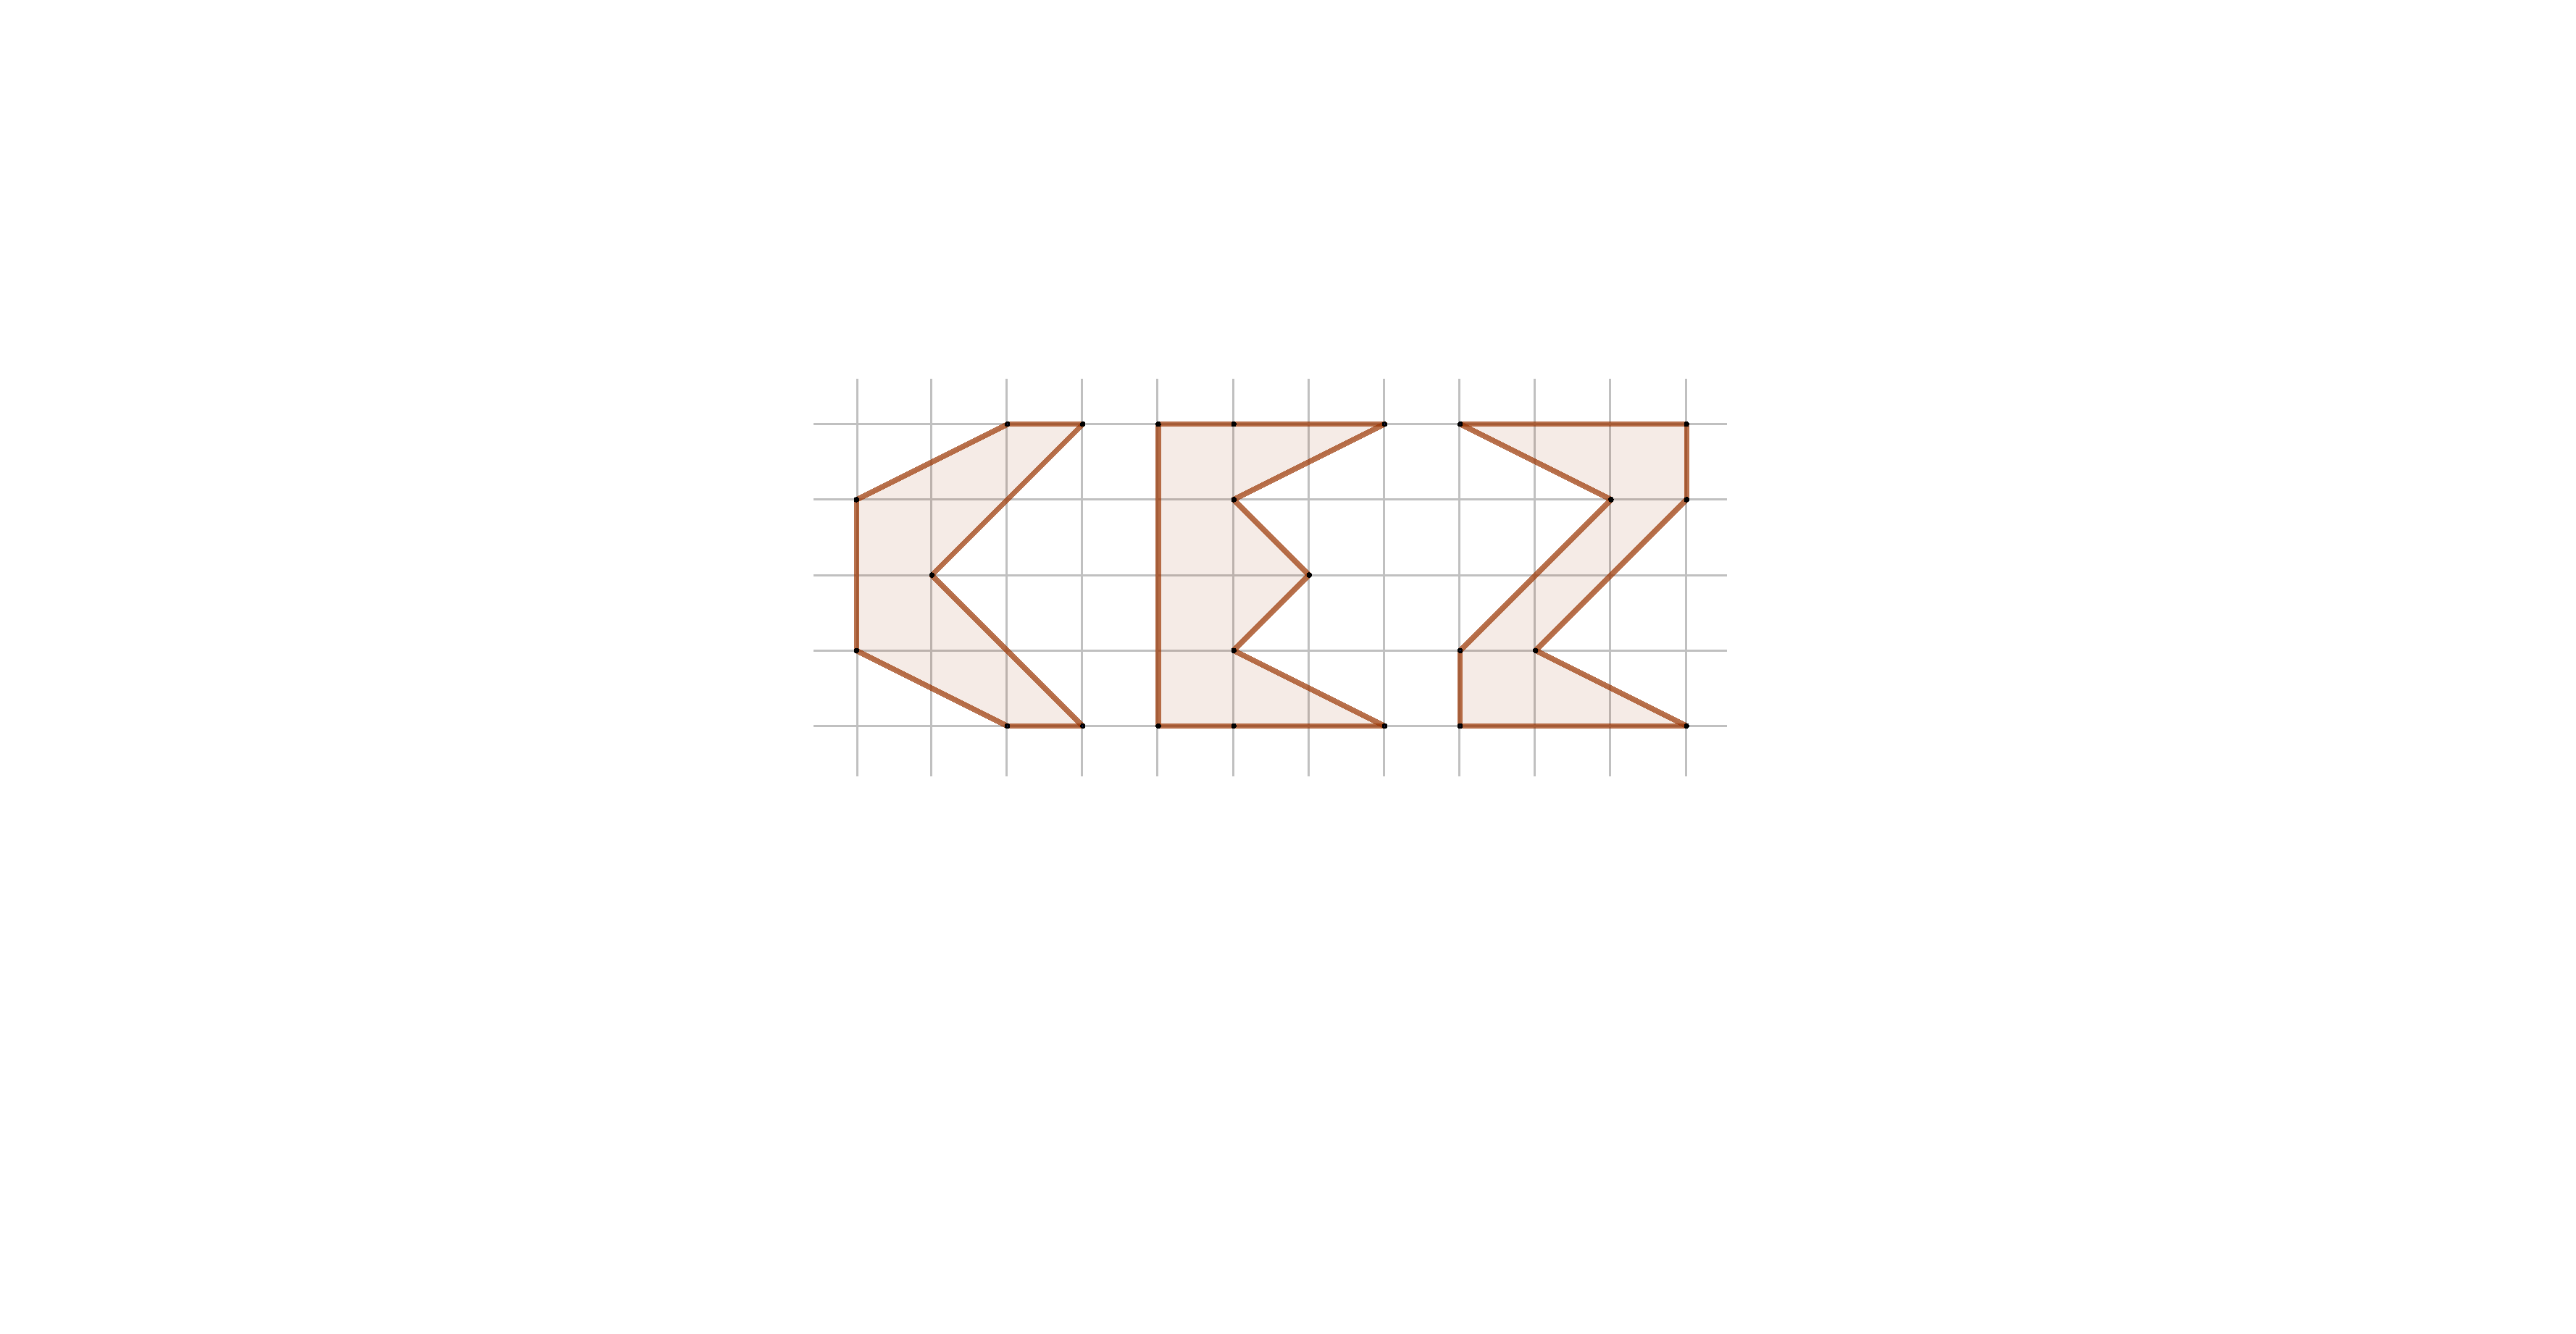
\includegraphics[width=0.6\textwidth]{úlohy/8/ctversit/11}

    \end{minipage}

    \item
    \begin{minipage}[t]{\linewidth}
        \begin{quote}
            Vypište všechny tvary, které jsou osově souměrné podle libovolné osy.
            Určete také součet obsahů tvarů C, H, F a G\@.
        \end{quote}
        \centering
        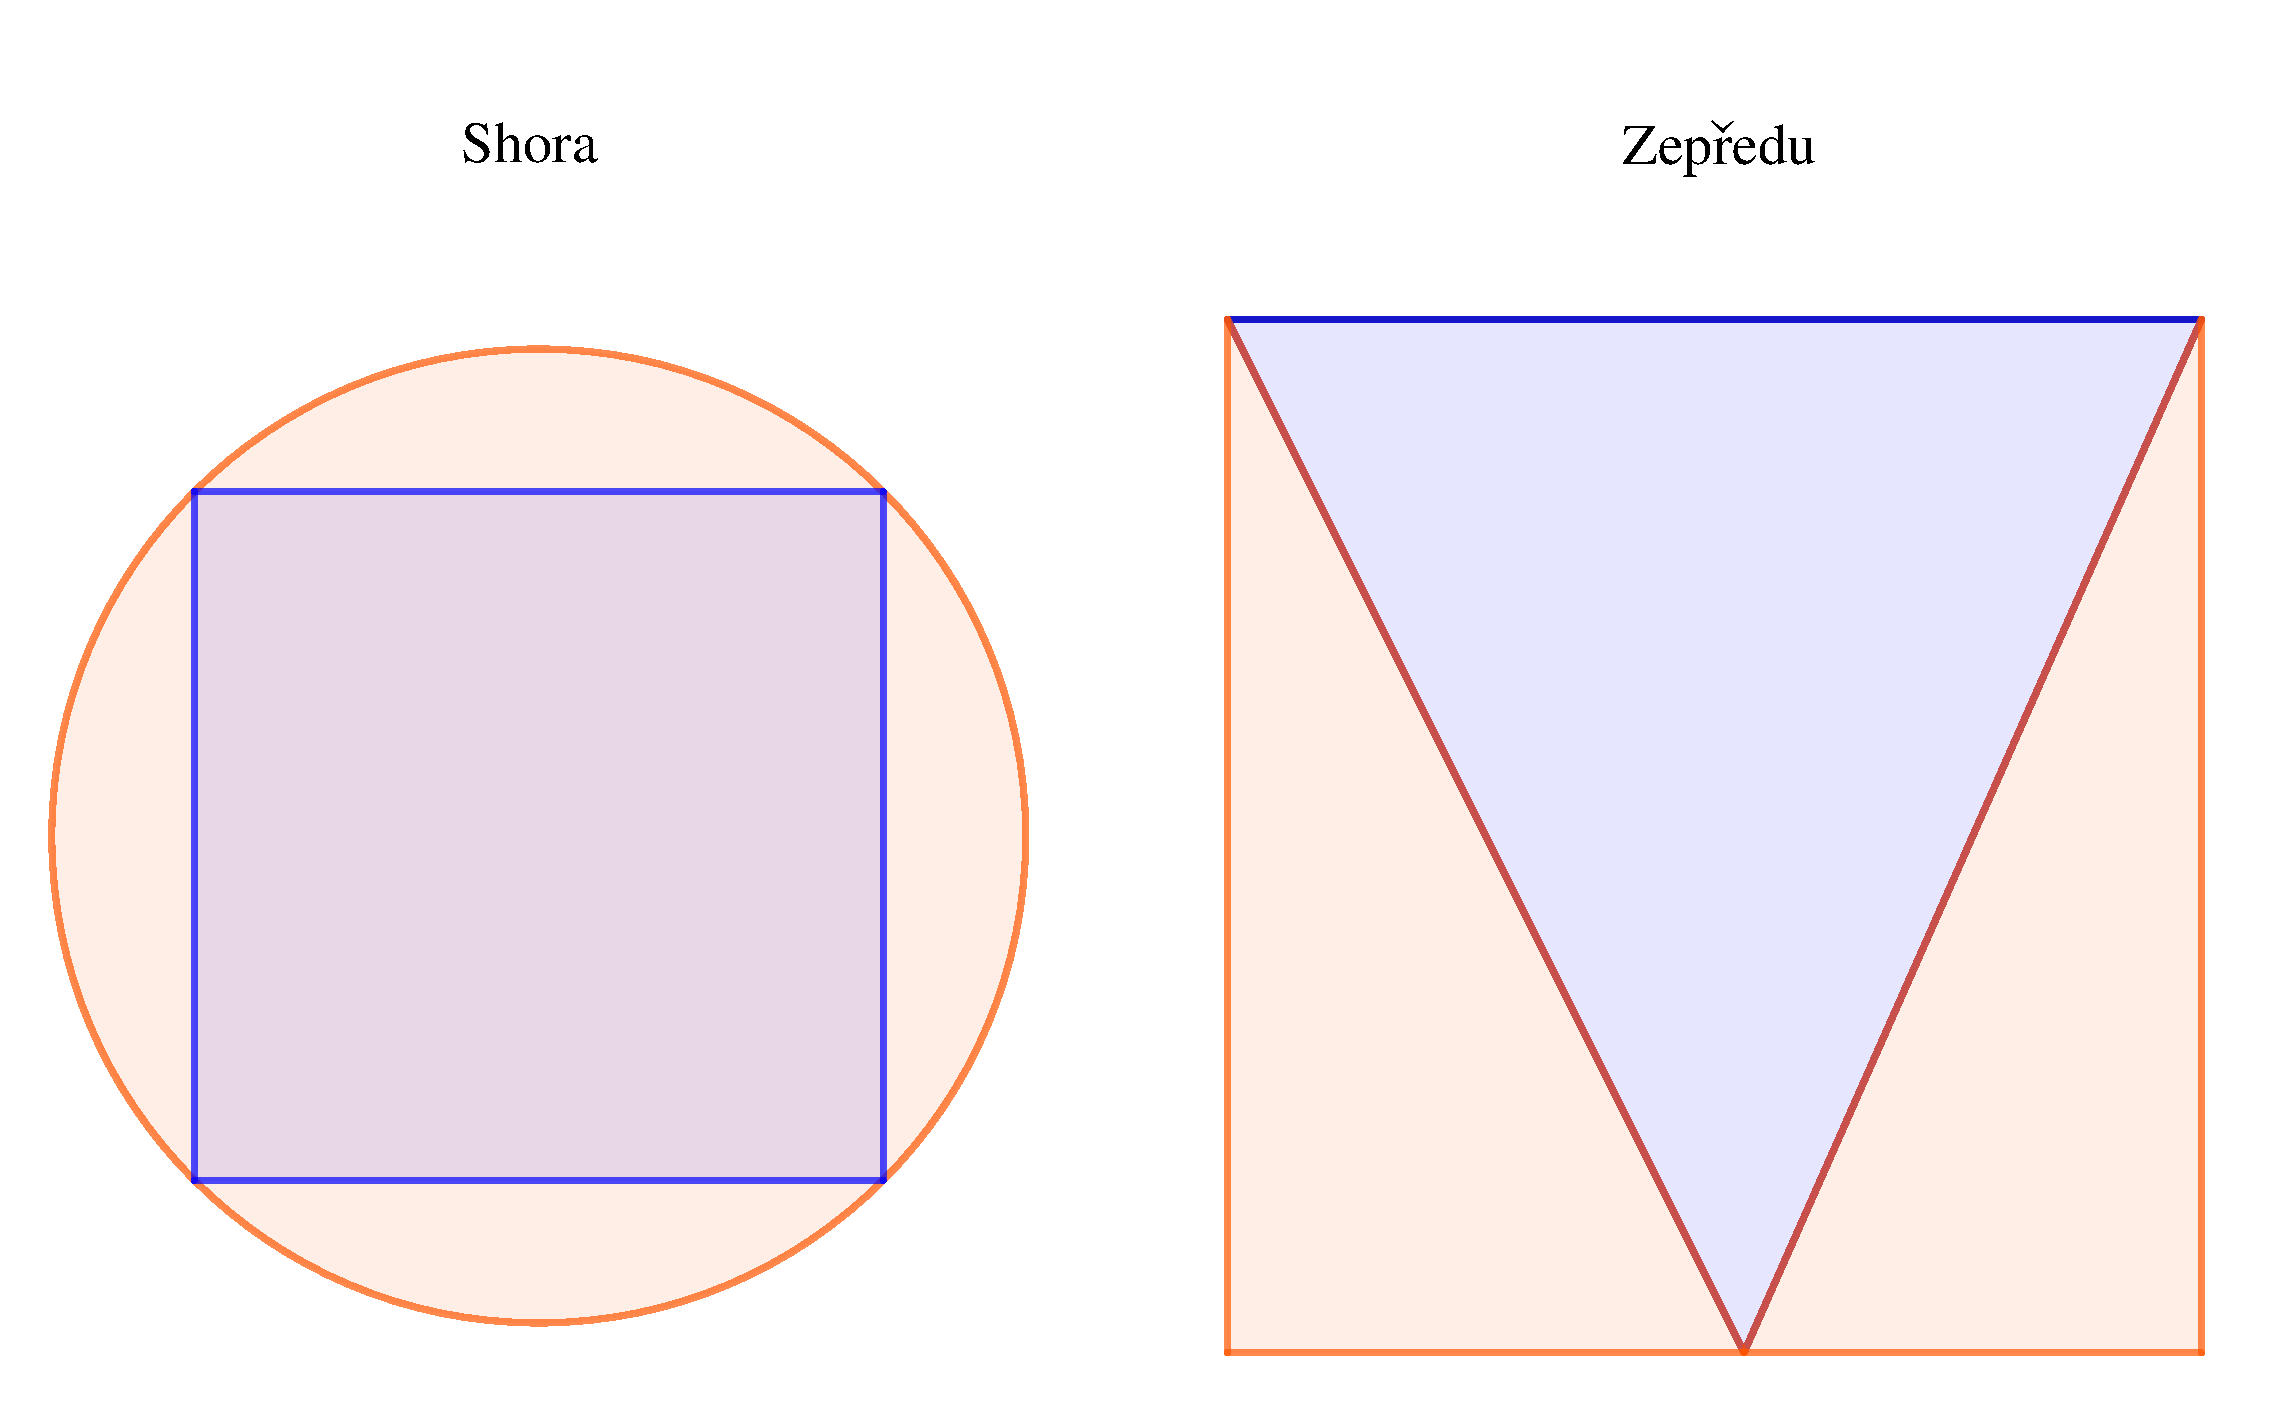
\includegraphics[width=0.7\textwidth]{úlohy/8/ctversit/12}

    \end{minipage}
\end{enumerate}

\newpage

\paragraph{Řešení}
\begin{enumerate}
    \item
    \begin{quote}
        Obsah $\triangle\text{DEF} = 7,5\,\text{cm}^2$, $\triangle\text{GCH} = 6\,\text{cm}^2$ a $\rectangle\text{ABCD} = 50\,\text{cm}^2$.
    \end{quote}

    \item
    \begin{quote}
        Obsah $\text{A} = 20\,\text{cm}^2$, $\text{B} = 21\,\text{cm}^2$.
    \end{quote}

    \item
    \begin{quote}
        Ano, ne, ano.
    \end{quote}

    \item
    \begin{quote}
        Oba mají stejný obsah, rozdíl je tedy $0\,\text{cm}^2$.
        Tvar A má obvod delší o 2 cm.
    \end{quote}

    \item
    \begin{quote}
        Obsah $\text{A} = 5\,\text{cm}^2$, $\text{B} = 2\,\text{cm}^2$, $\text{C} = 6\,\text{cm}^2$.
    \end{quote}

    \item
    \begin{quote}
        Pouze tvar A\@.
    \end{quote}

    \item
    \begin{quote}
        Obsah $\text{A} = 18\,\text{cm}^2$, $\text{B} = 18\,\text{cm}^2$, $\text{C} = 19\,\text{cm}^2$.
        Největší obsah má tvar C\@.
    \end{quote}

    \item
    \begin{quote}
        Obsah $\text{A} = 72\,\text{cm}^2$, $\text{B} = 80\,\text{cm}^2$, $\text{C} = 28\,\text{cm}^2$.
    \end{quote}

    \item
    \begin{quote}
        Oba tvary mají stejný obvod, rozdíl je tedy 0 cm.
        Obsah tvaru A je větší o $2\,\text{cm}^2$.
    \end{quote}

    \item
    \begin{quote}
        Obsah $\text{A} = 15,5\,\text{cm}^2$, $\text{B} = 8\,\text{cm}^2$, $\text{C} = 15\,\text{cm}^2$.
    \end{quote}

    \item
    \begin{quote}
        Součet obsahů je $25\,\text{cm}^2$.
        Obvod písmene Z je větší než obvod písmene C\@.
    \end{quote}

    \item
    \begin{quote}
        Tvary A, B, D, E, G a I jsou souměrné podle aspoň 1 osy.
        Součet obsahů je $15\,\text{cm}^2$.
    \end{quote}

\end{enumerate}

\newpage

\subsubsection{Obvod, obsah a délky}

\paragraph{Úlohy}
\begin{enumerate}
    \item
    \begin{minipage}[t]{\linewidth}
        \begin{quote}
            $\triangle$ABC je rovnostranný a $\triangle$ABD je rovnoramenný. $\lvert \text{BD} \rvert = 4\,\text{cm}$.
            Obvod $\triangle$ABD je 15 cm.
            Jaký je obvod tvaru ADBC?
        \end{quote}
        \centering
        \includegraphics[width=0.4\textwidth]{úlohy/8/obobde/1}

    \end{minipage}

    \item
    \begin{minipage}[t]{\linewidth}
        \begin{quote}
            $\triangle$ABD a $\triangle$ABE jsou rovnoramenné. $\lvert \text{AB} \rvert = 4\,\text{cm}$. $\lvert \text{AD} \rvert = 3\,\text{cm}$.
            Obvod $\triangle$ABE je 2krát delší než obvod $\triangle$ABD. Jaký je obvod tvaru ADBE?
        \end{quote}
        \centering
        \includegraphics[width=0.5\textwidth]{úlohy/8/obobde/2}

    \end{minipage}

    \item
    \begin{minipage}[t]{\linewidth}
        \begin{quote}
            $\triangle{\text{A}}_{1}$ a $\triangle{\text{A}}_{1}$ jsou navzájem shodné. $\triangle{\text{A}}_{1}$, $\triangle{\text{A}}_{1}$, $\triangle{\text{B}}$, $\triangle{\text{D}}$ jsou rovnostranné. $\triangle{\text{C}}$ je rovnoramenný.\             Obvod $\triangle{\text{A}}_{1}$ je 18 cm.
            Obvod $\triangle$D je o 3 cm delší než obvod $\triangle{\text{A}}_{1}$.
            Určete obvod $\triangle$C.
        \end{quote}
        \centering
        \includegraphics[width=0.45\textwidth]{úlohy/8/obobde/3}

    \end{minipage}

    \item
    \begin{minipage}[t]{\linewidth}
        \begin{quote}
            Z provázku byl sestrojen čtverec tak, že byl provázek natažen po jeho obvodu.
            Jeho obsah je $49\,\text{cm}^{2}$.
            Poté byl tento provázek rozmotán, a byl z něj vytvořen obdélník o obsahu $45\,\text{cm}^{2}$.
            Jaké jsou délky jeho stran?
            (Obrázek je pouze ilustrační)
        \end{quote}
        \centering
        \includegraphics[width=0.6\textwidth]{úlohy/8/obobde/4}

    \end{minipage}

    \item
    \begin{minipage}[t]{\linewidth}
        \begin{quote}
            Tvar vlevo má obvod 182 cm.
            Skládá se z malých a velkých čtverců.\ 4 malé čtverce se vejdou do jednoho velkého.
            Určete obvody tvaru uprostřed a vpravo.
        \end{quote}
        \centering
        \includegraphics[width=0.8\textwidth]{úlohy/8/obobde/5}

    \end{minipage}

    \item
    \begin{minipage}[t]{\linewidth}
        \begin{quote}
            Obvod malého modrého obdélníku je 72 cm.
            Jeho delší strana je 2krát delší než jeho kratší strana.
            Tvar vpravo je čtverec.
            Určete obsah prostředního tvaru.
        \end{quote}
        \centering
        \includegraphics[width=0.7\textwidth]{úlohy/8/obobde/6}

    \end{minipage}

    \item
    \begin{minipage}[t]{\linewidth}
        \begin{quote}
            Obvod $\rectangle$A je 34 cm.
            Obsah $\rectangle$B je $35\,\text{cm}^{2}$.
            Jaké jsou délky stran $\rectangle$A?
        \end{quote}
        \centering
        \includegraphics[width=0.7\textwidth]{úlohy/8/obobde/7}

    \end{minipage}

    \item
    \begin{minipage}[t]{\linewidth}
        \begin{quote}
            Zelené $\triangle$ jsou rovnostranné a pravoúhlé.
            Obvod tvaru A je 77~cm, obvod tvaru B je 82 cm.
            Jaká je délka základny zeleného $\triangle$?
        \end{quote}
        \centering
        \includegraphics[width=0.7\textwidth]{úlohy/8/obobde/8}

    \end{minipage}

    \item
    \begin{minipage}[t]{\linewidth}
        \begin{quote}
            Délka $\overline{\text{g}}$ je 14 cm.
            Jaký je obsah čtverce D?
        \end{quote}
        \centering
        \includegraphics[width=0.7\textwidth]{úlohy/8/obobde/9}

    \end{minipage}

    \item
    \begin{minipage}[t]{\linewidth}
        \begin{quote}
            Obsah $\square$ABCD je 64 cm.
            Obvod $\triangle$ABF je 2krát delší než obvod $\square$ABCD. Součet délek obou ramen $\triangle$ABF se rovná obvodu $\triangle$CDE. Jaký je obvod tvaru EDAFBC?
        \end{quote}
        \centering
        \includegraphics[width=0.7\textwidth]{úlohy/8/obobde/10}

    \end{minipage}
\end{enumerate}


\newpage

\paragraph{Řešení}
\begin{enumerate}
    \item
    \begin{quote}
        Obvod tvaru ADBC je 22 cm.
    \end{quote}

    \item
    \begin{quote}
        Obvod tvaru ADBE je 22 cm.
    \end{quote}

    \item
    \begin{quote}
        Obvod $\triangle$C je 31 cm.
    \end{quote}

    \item
    \begin{quote}
        Délky stran jsou 9 cm a 5 cm.
    \end{quote}

    \item
    \begin{quote}
        Obvod tvaru uprostřed je 312 cm.
        Obvod tvaru vpravo je 130 cm.
    \end{quote}

    \item
    \begin{quote}
        Obsah prostředního tvaru je $216\,\text{cm}^{2}$.
    \end{quote}

    \item
    \begin{quote}
        Délky stran jsou 10 cm a 7 cm.
    \end{quote}

    \item
    \begin{quote}
        Délka základny zeleného $\triangle$ je 5 cm.
    \end{quote}

    \item
    \begin{quote}
        Obsah $\square$D je $4\,\text{cm}^{2}$.
    \end{quote}

    \item
    \begin{quote}
        Obvod tvaru EDAFBC je 120 cm?
    \end{quote}
\end{enumerate}

\newpage

\subsubsection{Rekurzivní úlohy}
Úlohy zaměřené na opakování jevů.

\paragraph{Úlohy}
\begin{enumerate}
    \item
    \begin{minipage}[t]{\linewidth}
        \begin{quote}
            Na obrázku je vyobrazen květ rostliny, který má 4 okvětní lístky. Každý den se každý okvětní lístek prodlouží o jednu sekci. Vlevo je květ v první den, vpravo druhý den. Jedna sekce okvětního lístku má povrch 4 cm$^{2}$.

            Kolik bude mít květ okvětních lístků den 15.? Kolik budou mít každý sekcí? Jaký bude celkový povrch lístků? (Do tohoto součtu nepočítejte střed květu)
        \end{quote}
        \centering
        \includegraphics[width=0.7\textwidth]{úlohy/8/rekur/1}
    \end{minipage}

    \item
    \begin{minipage}[t]{\linewidth}
        \begin{quote}
            Na obrázku je krystal ve 3 fázích růstu, a to v prvním, druhém a třetím roce. Každý rok na konce krystalu (vrcholy $\triangle$) které jsou „volné” přibude další $\triangle$. Ten bude mít poloviční povrch než $\triangle$, ze kterého roste.

            Z kolika $\triangle$ se bude krystal skládat v den 8? Pokud má krystal první rok povrch o velikosti 32 cm$^{2}$, jaký bude mít povrch v 6.~roce?
        \end{quote}
        \centering
        \includegraphics[width=0.6\textwidth]{úlohy/8/rekur/2}
    \end{minipage}

    \item
    \begin{minipage}[t]{\linewidth}
        \begin{quote}
            Včelky budují plástev. Staví jí tak, že každou hodinu přidají jedno patro, ale pouze směrem nahoru. Na obrázku je postup jejich stavby v hodině 1., 2., a 3. zleva doprava. Do většiny komůrek je uložen med (vyznačen oranžově), některé jsou ale ponechané prázdné. Tyto prázdné komůrky jsou vždy odděleny ze všech stran medem.

            Kolik komůrek bude plástev mít ve 12. hodině? Kolik prázdných komůrek bude mít v hodině 6.?
        \end{quote}
        \centering
        \includegraphics[width=0.7\textwidth]{úlohy/8/rekur/3}
    \end{minipage}

    \item
    \begin{minipage}[t]{\linewidth}
        \begin{quote}
            Na prvním obrázku jsou 3 přímky, které se všechny navzájem protínají. Do dalšího, druhého, obrázku je na každý průsečík narýsována přímka, která je $\perp$ s přímkou která průsečík netvoří. Tímto systémem se pokračuje dál.

            Kolik průsečíků vznikne na dalším, 4. obrázku?
        \end{quote}
        \centering
        \includegraphics[width=0.8\textwidth]{úlohy/8/rekur/4}
    \end{minipage}

    \item
    \begin{minipage}[t]{\linewidth}
        \begin{quote}
            Na obrázku je vyobrazen had. Každý týden povyroste o jedno zatočení kolem svého těla. Vlevo nahoře je had v první týden, vpravo nahoře v týden druhý a uprostřed dole v týden třetí.

            Pokud je had v prvním týdnu dlouhý 6 cm, jak dlouhý bude v~týdnu 4. a 5.?
        \end{quote}
        \centering
        \includegraphics[width=0.6\textwidth]{úlohy/8/rekur/5}
    \end{minipage}

    \item
    \begin{minipage}[t]{\linewidth}
        \begin{quote}
            Na obrázku je vesnice, která se každý rok rozroste. Domy vždy přibudou tak, že všechny domy z předchozího roku budou mít sousedy ze všech světových stran.

            Kolik bude domů mezi domem prostředním a nejsevernějším domem v roce 100? (prostřední a nejsevernější dům nepočítejte)
            
            Z kolika domů se bude vesnice skládat ve 20. rok?
        \end{quote}
        \centering
        \includegraphics[width=0.5\textwidth]{úlohy/8/rekur/6}
    \end{minipage}


\end{enumerate}

\newpage

\paragraph{Řešení}
\begin{enumerate}
    \item
    \begin{quote}
        15. den bude mít stále 4 okvětní lístky. Každý bude mít 15 sekcí. Celkový povrch bude 240 cm$^{2}$.
    \end{quote}

    \item
    \begin{quote}
        V den 8. se bude skládat z 384 lístků. Povrch v den 6. bude 3008~cm$^{2}$.
    \end{quote}

    \item
    \begin{quote}
        Ve 12. hodině bude mít 102 komůrek. V 6. hodině bude mít 12 prázdných komůrek.
    \end{quote}

    \item
    \begin{quote}
        Vznikne 30 nových průsečíků.
    \end{quote}

    \item
    \begin{quote}
        V 4. týdnu bude měřit 123 cm, v 5. 200 cm.
    \end{quote}

    \item
    \begin{quote}
        Bude mezi nimi 98 domů. Ve 20. rok se bude skládat z 761 domů.
    \end{quote}
\end{enumerate}

\newpage

\subsection{Rýsování}
\label{subsec:rysovani}

\subsubsection{Podle bodů}

\paragraph{Úlohy}
\begin{enumerate}
    \item
    \begin{minipage}[t]{\linewidth}
        \begin{quote}
            Narýsujte $\square$ABED tak, aby v něm ležel bod C. Dále sestrojte $\triangle$DCE\@.
        \end{quote}
        \centering
        \includegraphics[width=\textwidth]{úlohy/8/rysovani/b/1}

    \end{minipage}

    \item
    \begin{minipage}[t]{\linewidth}
        \begin{quote}
            Narýsujte $\rectangle$ACDE tak, aby na $\overleftrightarrow{\text{ED}}$ ležel bod B\@.
        \end{quote}
        \centering
        \includegraphics[width=\textwidth]{úlohy/8/rysovani/b/2}

    \end{minipage}

    \item
    \begin{minipage}[t]{\linewidth}
        \begin{quote}
            Narýsujte $\square$ADEF. Bod D leží na $\overline{\text{AB}}$ a bod E leží na $\overline{\text{DC}}$. $\angle$ABD tedy musí být pravý.
        \end{quote}
        \centering
        \includegraphics[width=\textwidth]{úlohy/8/rysovani/b/3}

    \end{minipage}

    \item
    \begin{minipage}[t]{\linewidth}
        \begin{quote}
            Narýsujte $\square$BCDE tak, aby se v něm nenacházel bod A. Následovně narýsujte bod A', který je osově souměrný bodu A dle $\overline{\text{BC}}$.
            Poté sestrojte $\triangle$AA'B.
        \end{quote}
        \centering
        \includegraphics[width=\textwidth]{úlohy/8/rysovani/b/4}

    \end{minipage}

    \item
    \begin{minipage}[t]{\linewidth}
        \begin{quote}
            Narýsujte $\rectangle$ABDE tak, aby $\lvert \overline{\text{BC}} \rvert$ = $\lvert \overline{\text{CD}} \rvert$.
        \end{quote}
        \centering
        \includegraphics[width=\textwidth]{úlohy/8/rysovani/b/5}

    \end{minipage}

    \item
    \begin{minipage}[t]{\linewidth}
        \begin{quote}
            Narýsujte $\rectangle$BCDF tak, aby $\lvert \overline{\text{AB}} \rvert$ = $\lvert \overline{\text{AD}} \rvert$.
            Sestrojte všechny možnosti.
        \end{quote}
        \centering
        \includegraphics[width=\textwidth]{úlohy/8/rysovani/b/6}

    \end{minipage}
\end{enumerate}


\newpage

\paragraph{Řešení}
\begin{enumerate}
    \item
    \begin{minipage}[t]{\linewidth}
        \begin{quote}
            \phantom{text}
        \end{quote}
        \centering
        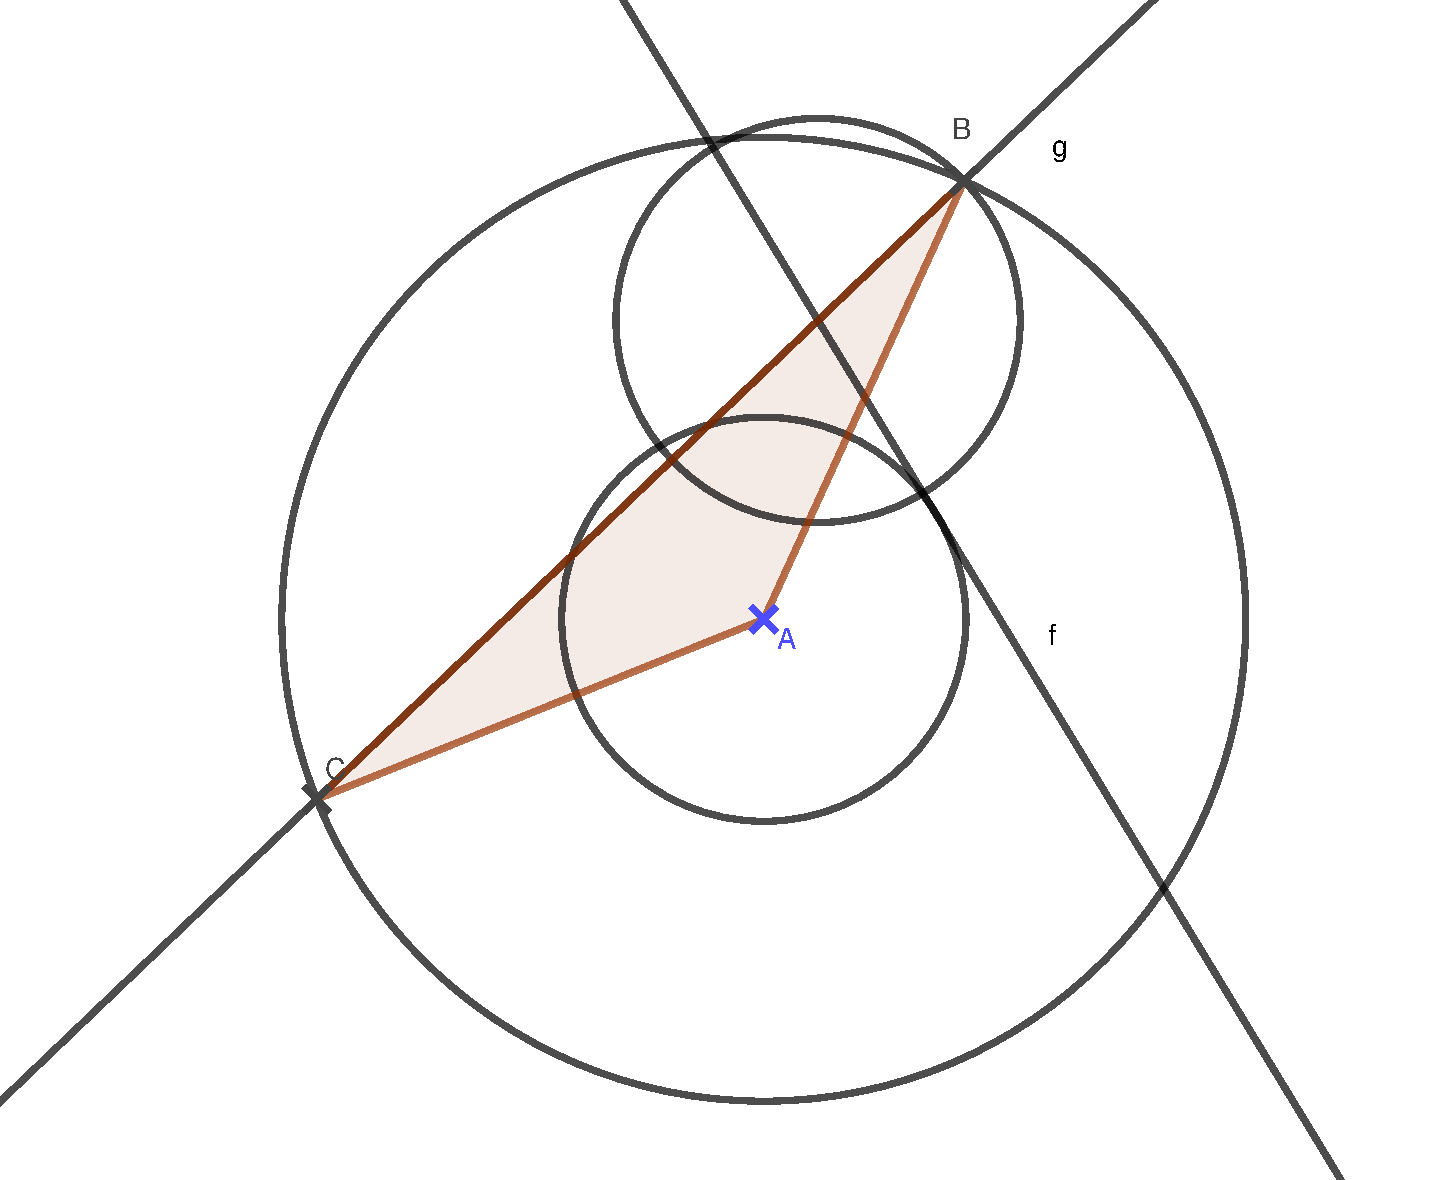
\includegraphics[width=0.5\textwidth]{úlohy/8/rysovani/b/1-v}

    \end{minipage}

    \item
    \begin{minipage}[t]{\linewidth}
        \begin{quote}
            \phantom{text}
        \end{quote}
        \centering
        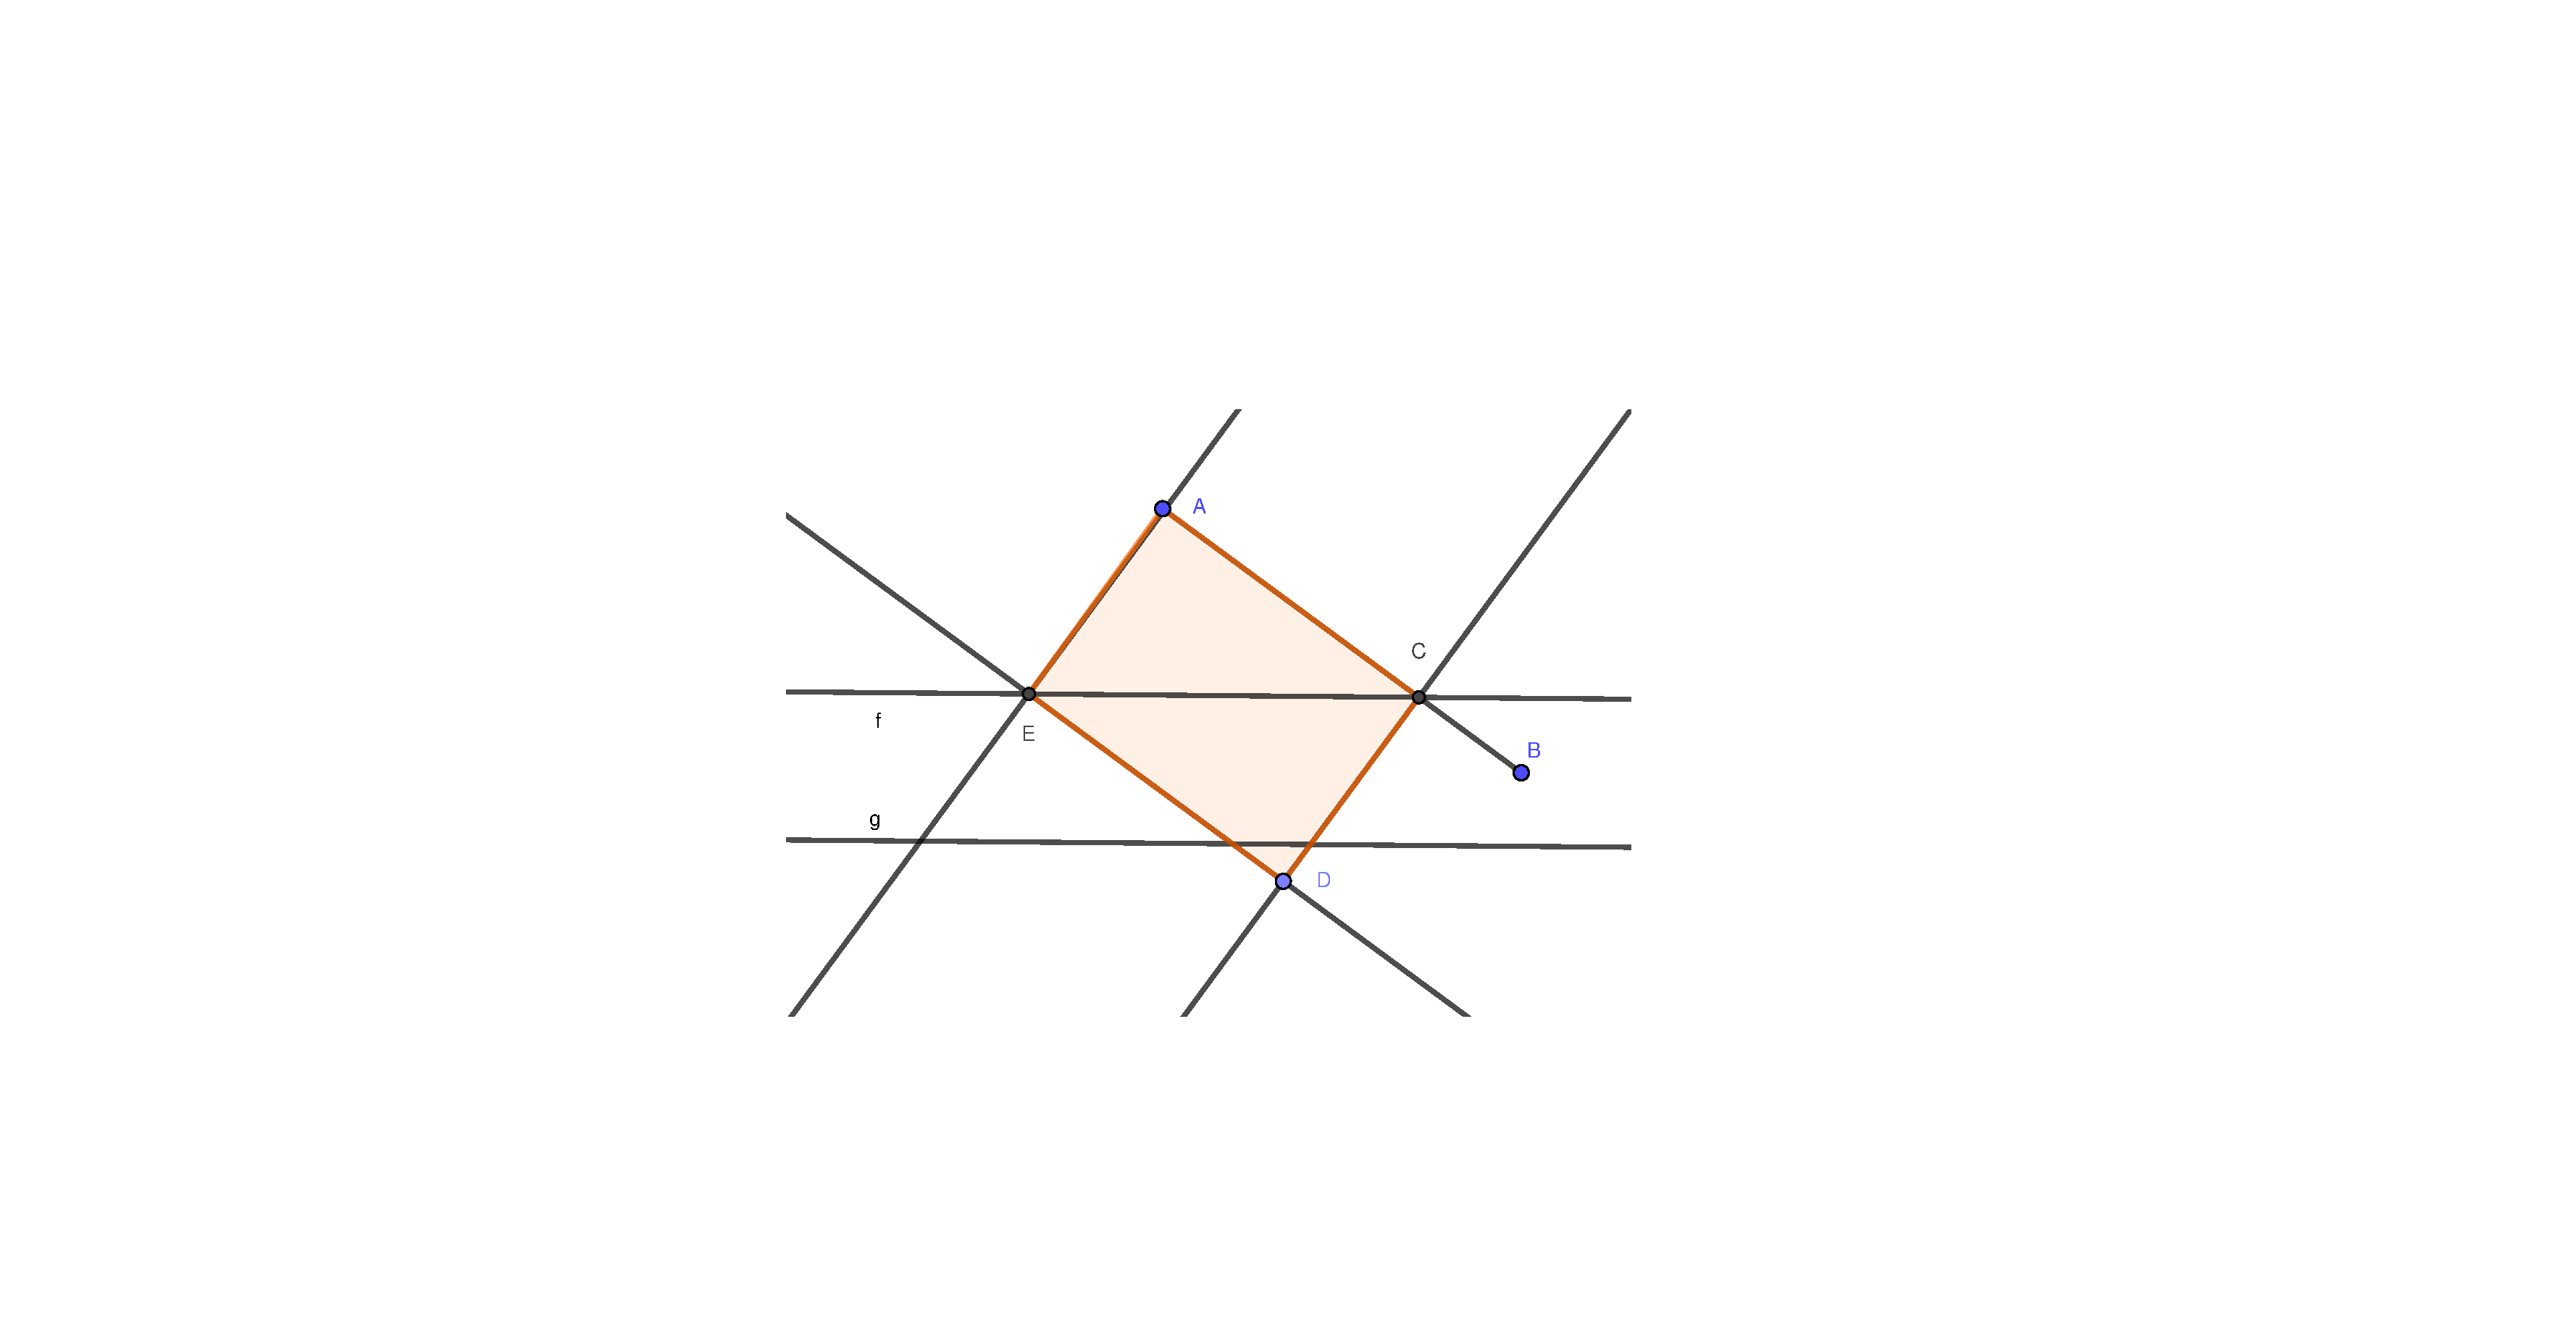
\includegraphics[width=0.7\textwidth]{úlohy/8/rysovani/b/2-v}

    \end{minipage}

    \item
    \begin{minipage}[t]{\linewidth}
        \begin{quote}
            \phantom{text}
        \end{quote}
        \centering
        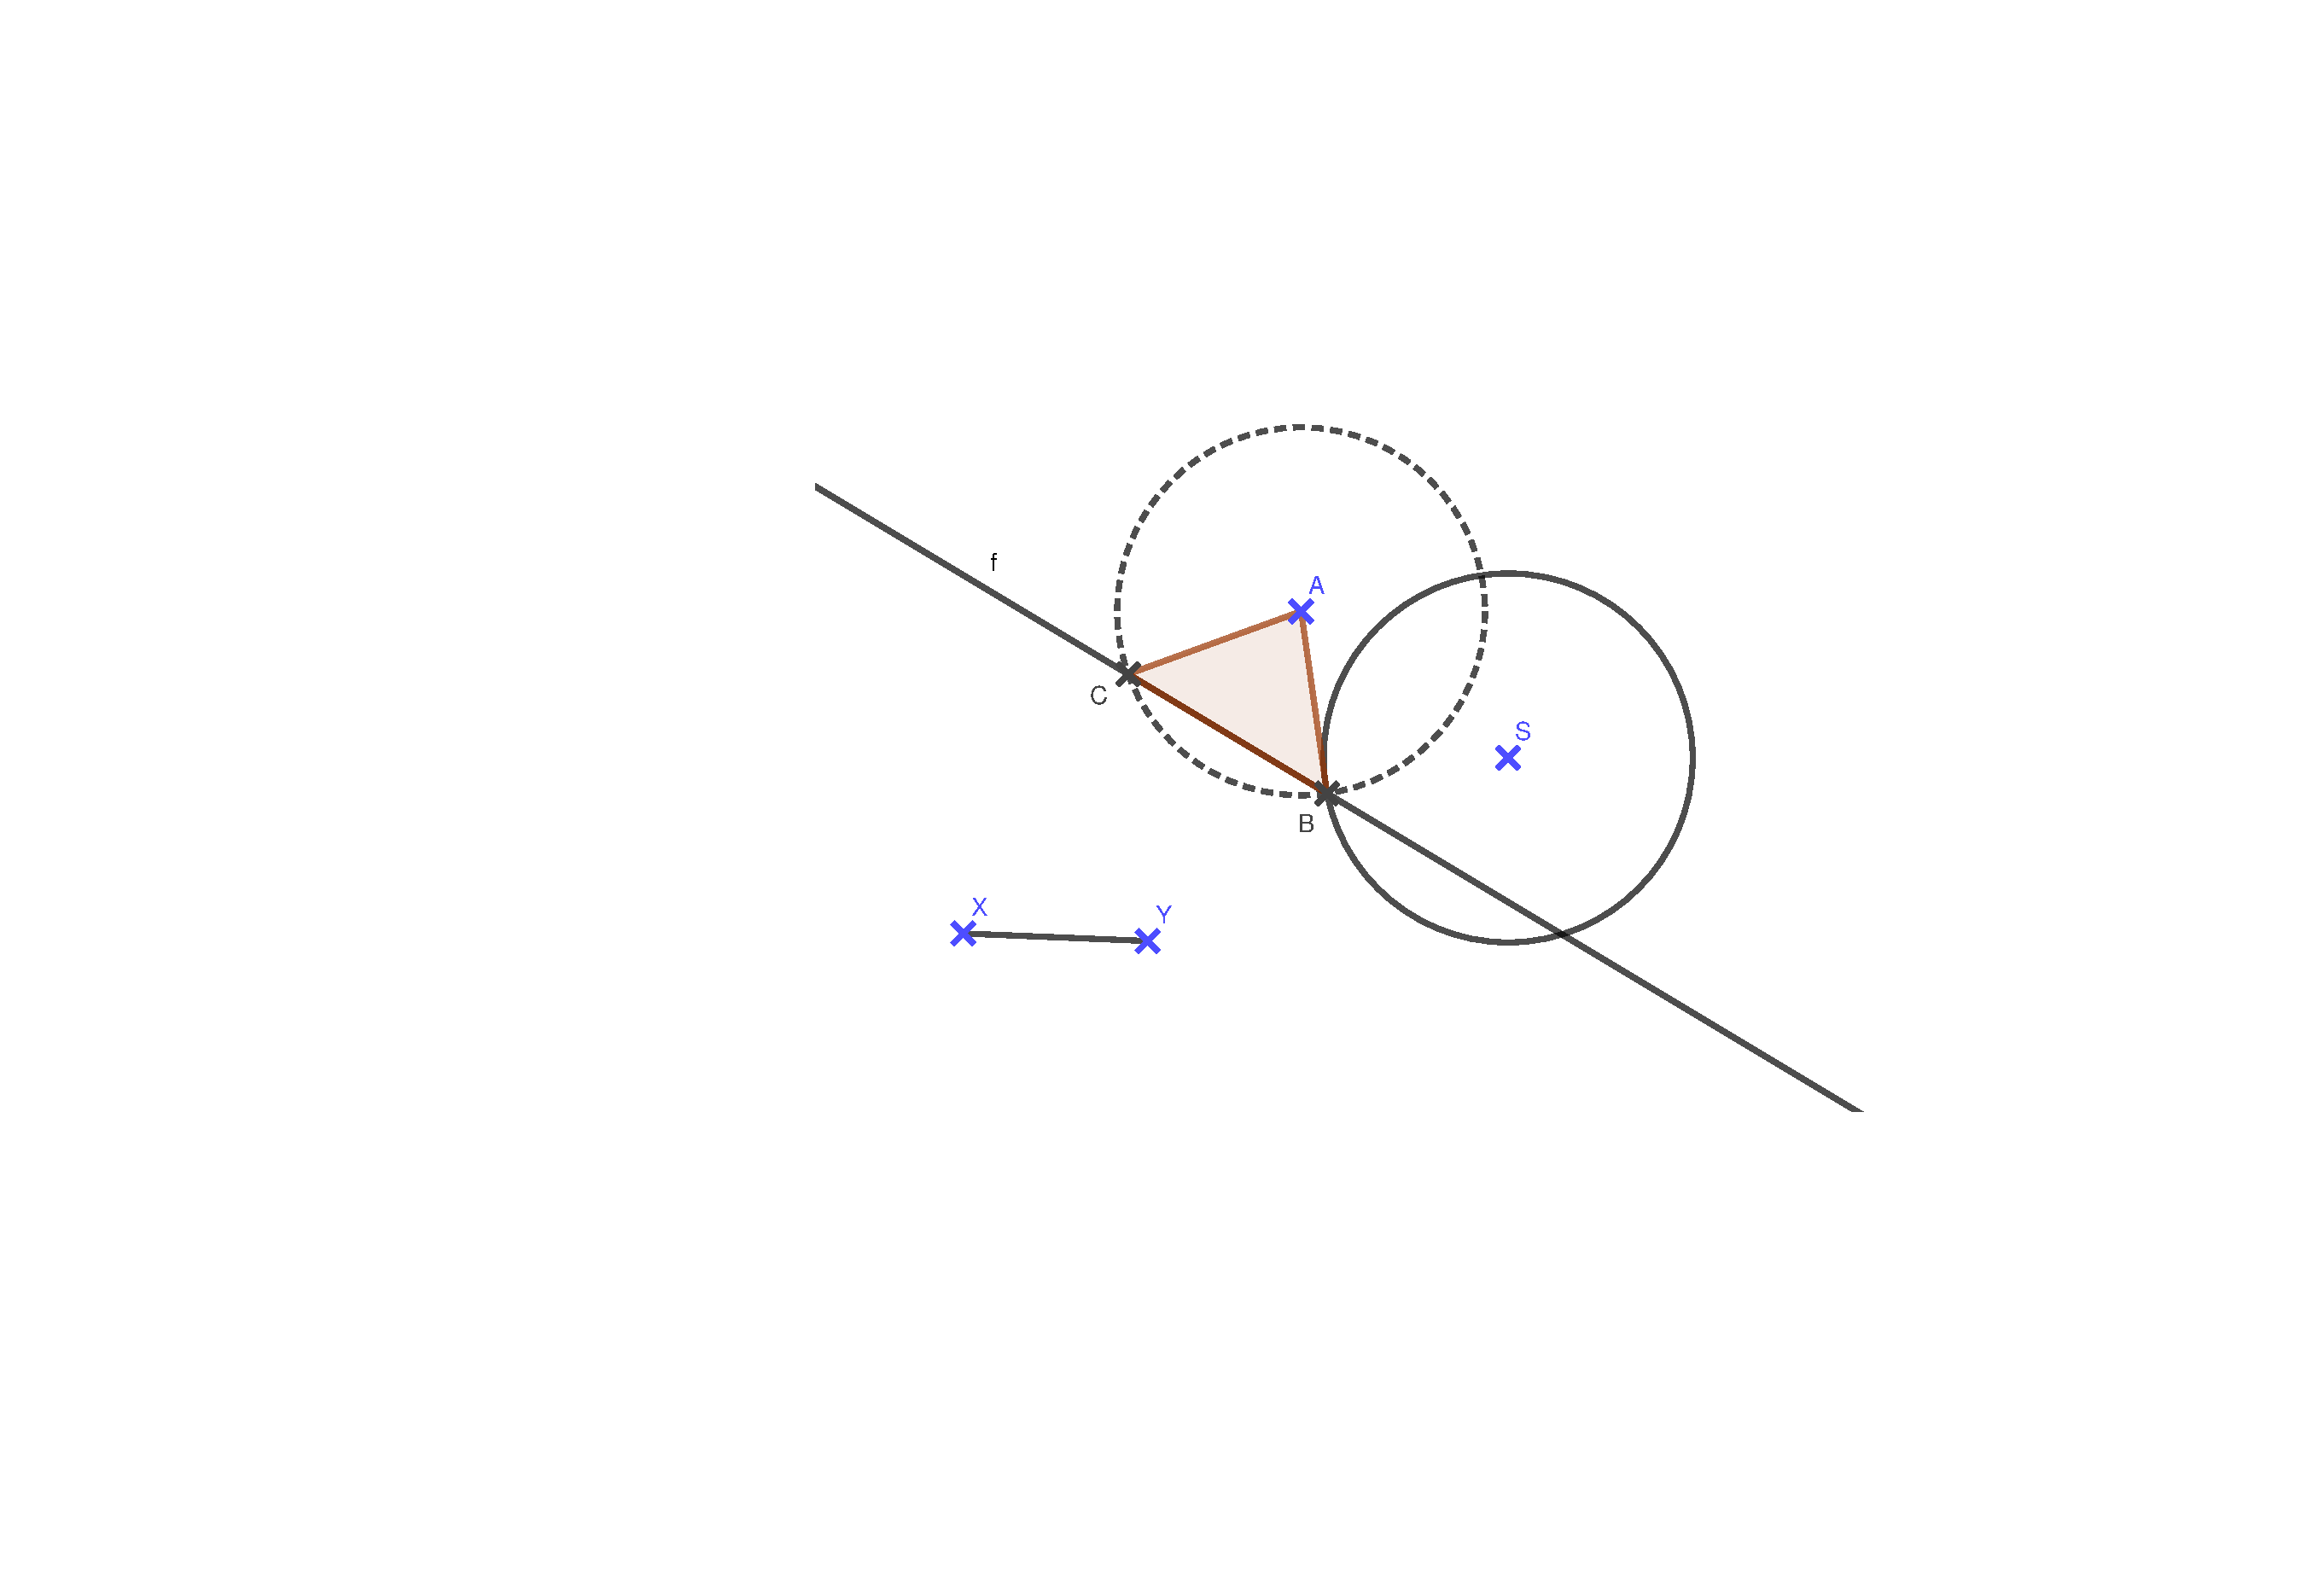
\includegraphics[width=0.8\textwidth]{úlohy/8/rysovani/b/3-v}

    \end{minipage}

    \item
    \begin{minipage}[t]{\linewidth}
        \begin{quote}
            \phantom{text}
        \end{quote}
        \centering
        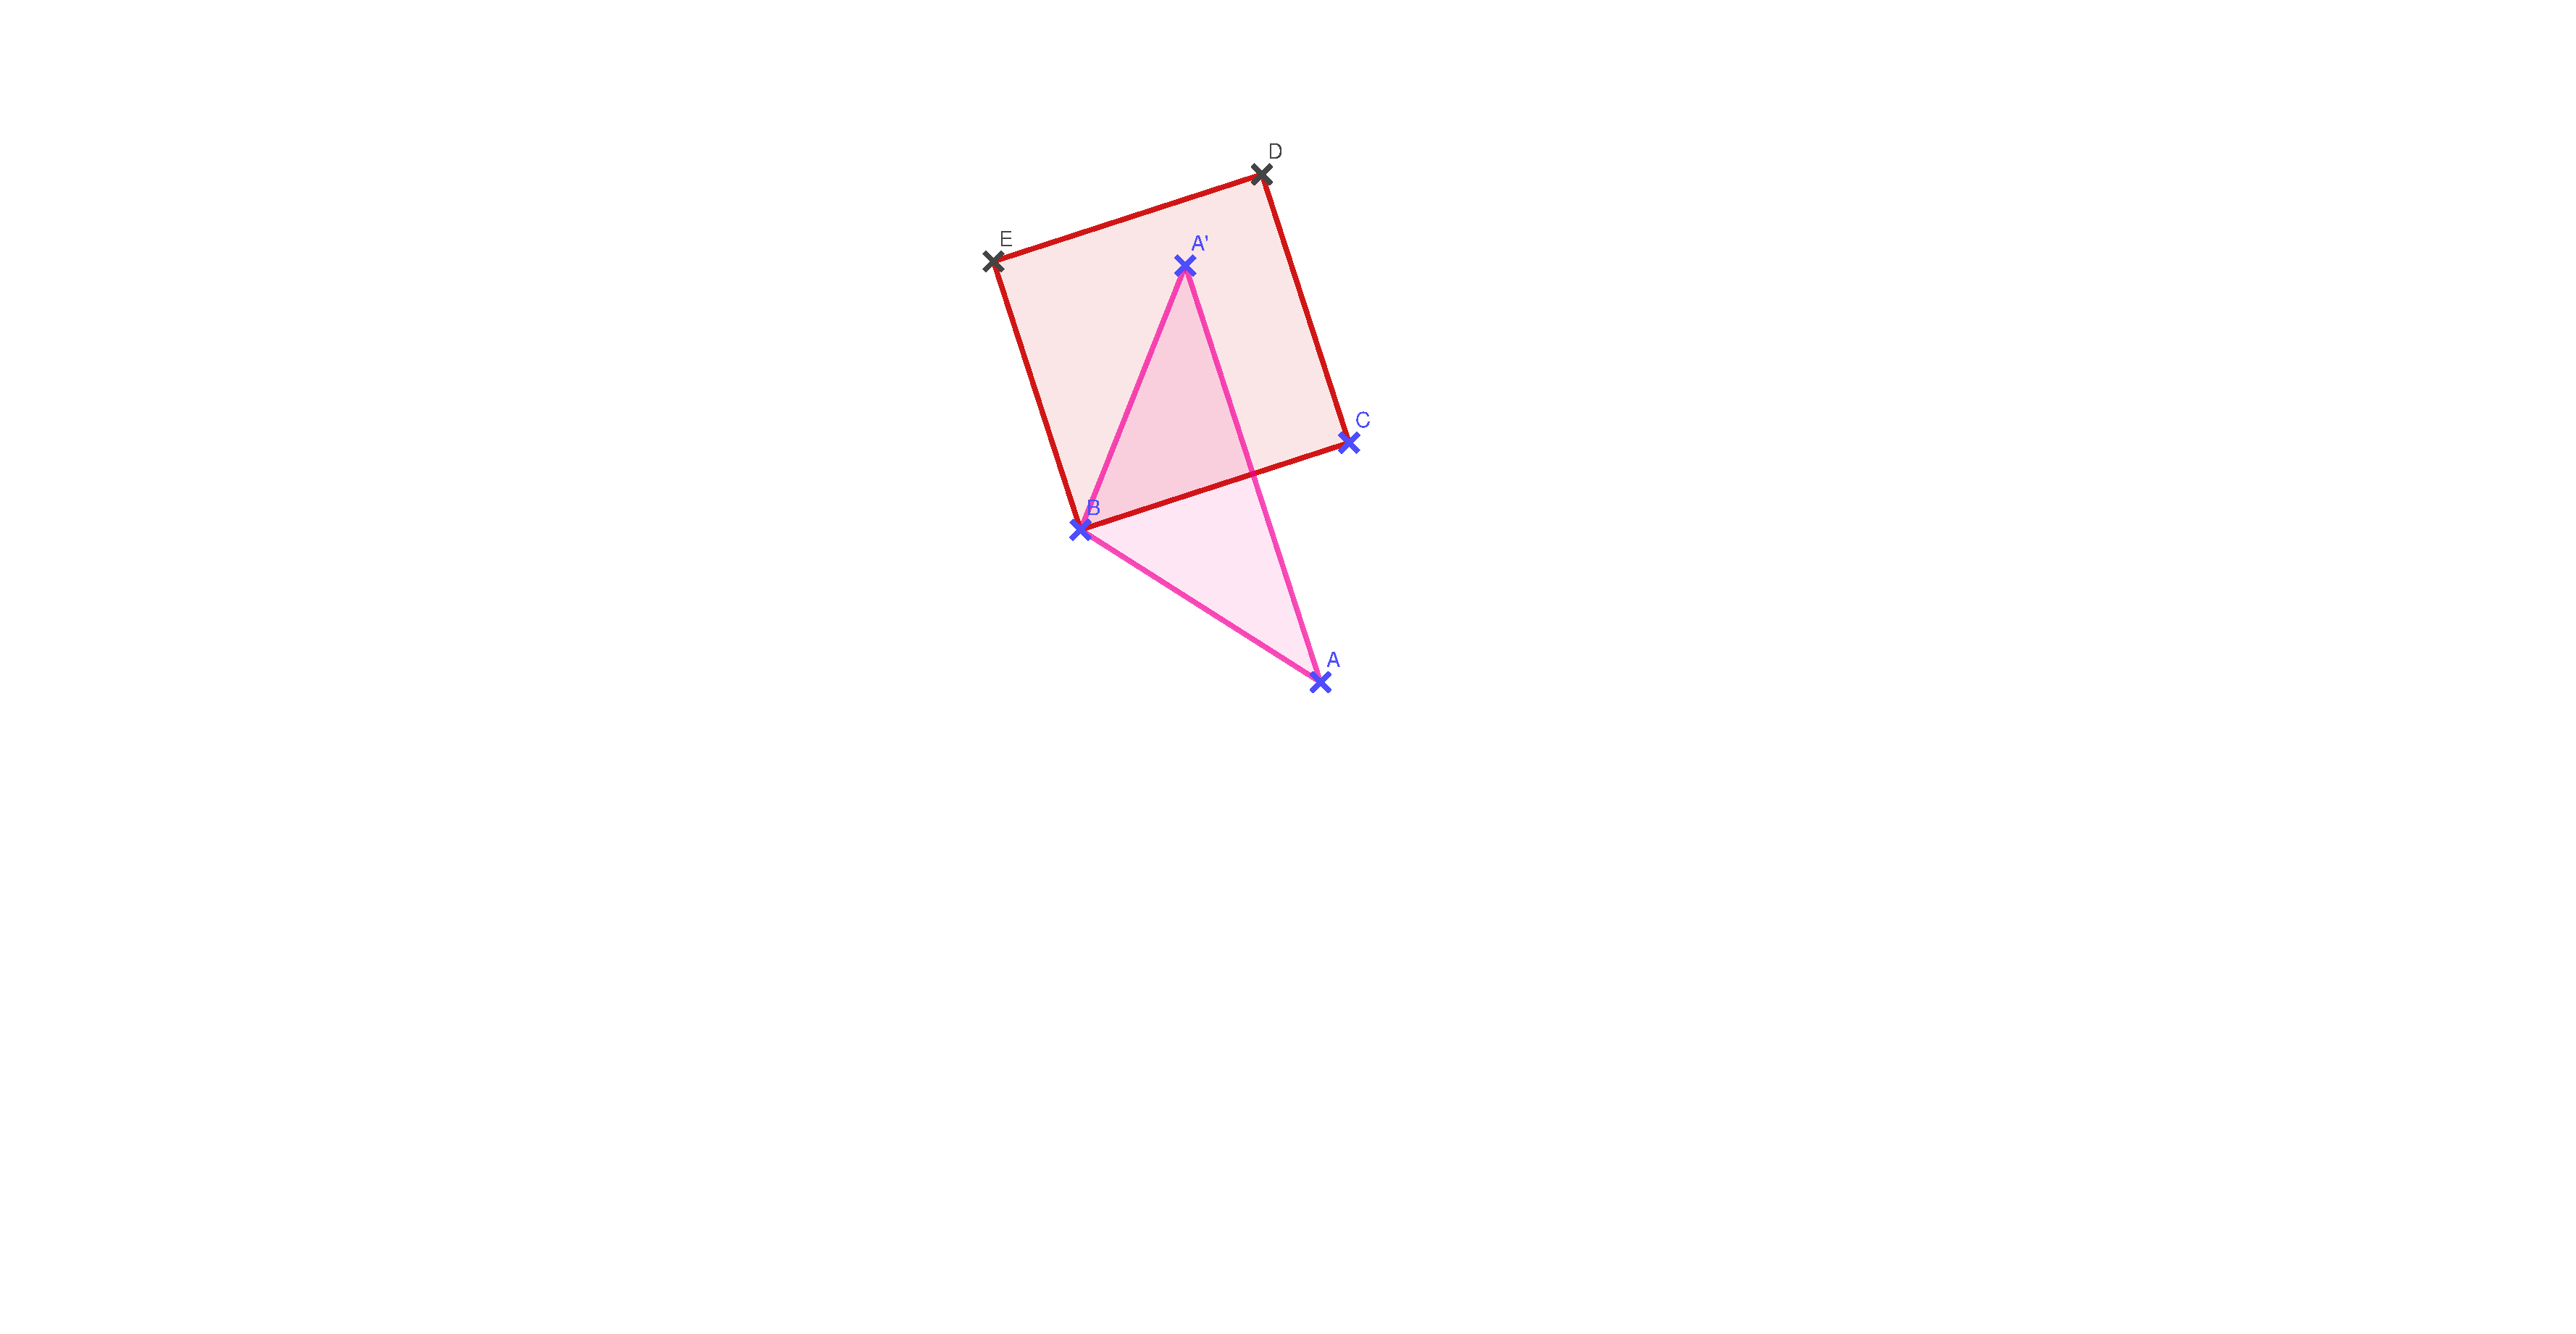
\includegraphics[width=0.7\textwidth]{úlohy/8/rysovani/b/4-v}

    \end{minipage}

    \item
    \begin{minipage}[t]{\linewidth}
        \begin{quote}
            \phantom{text}
        \end{quote}
        \centering
        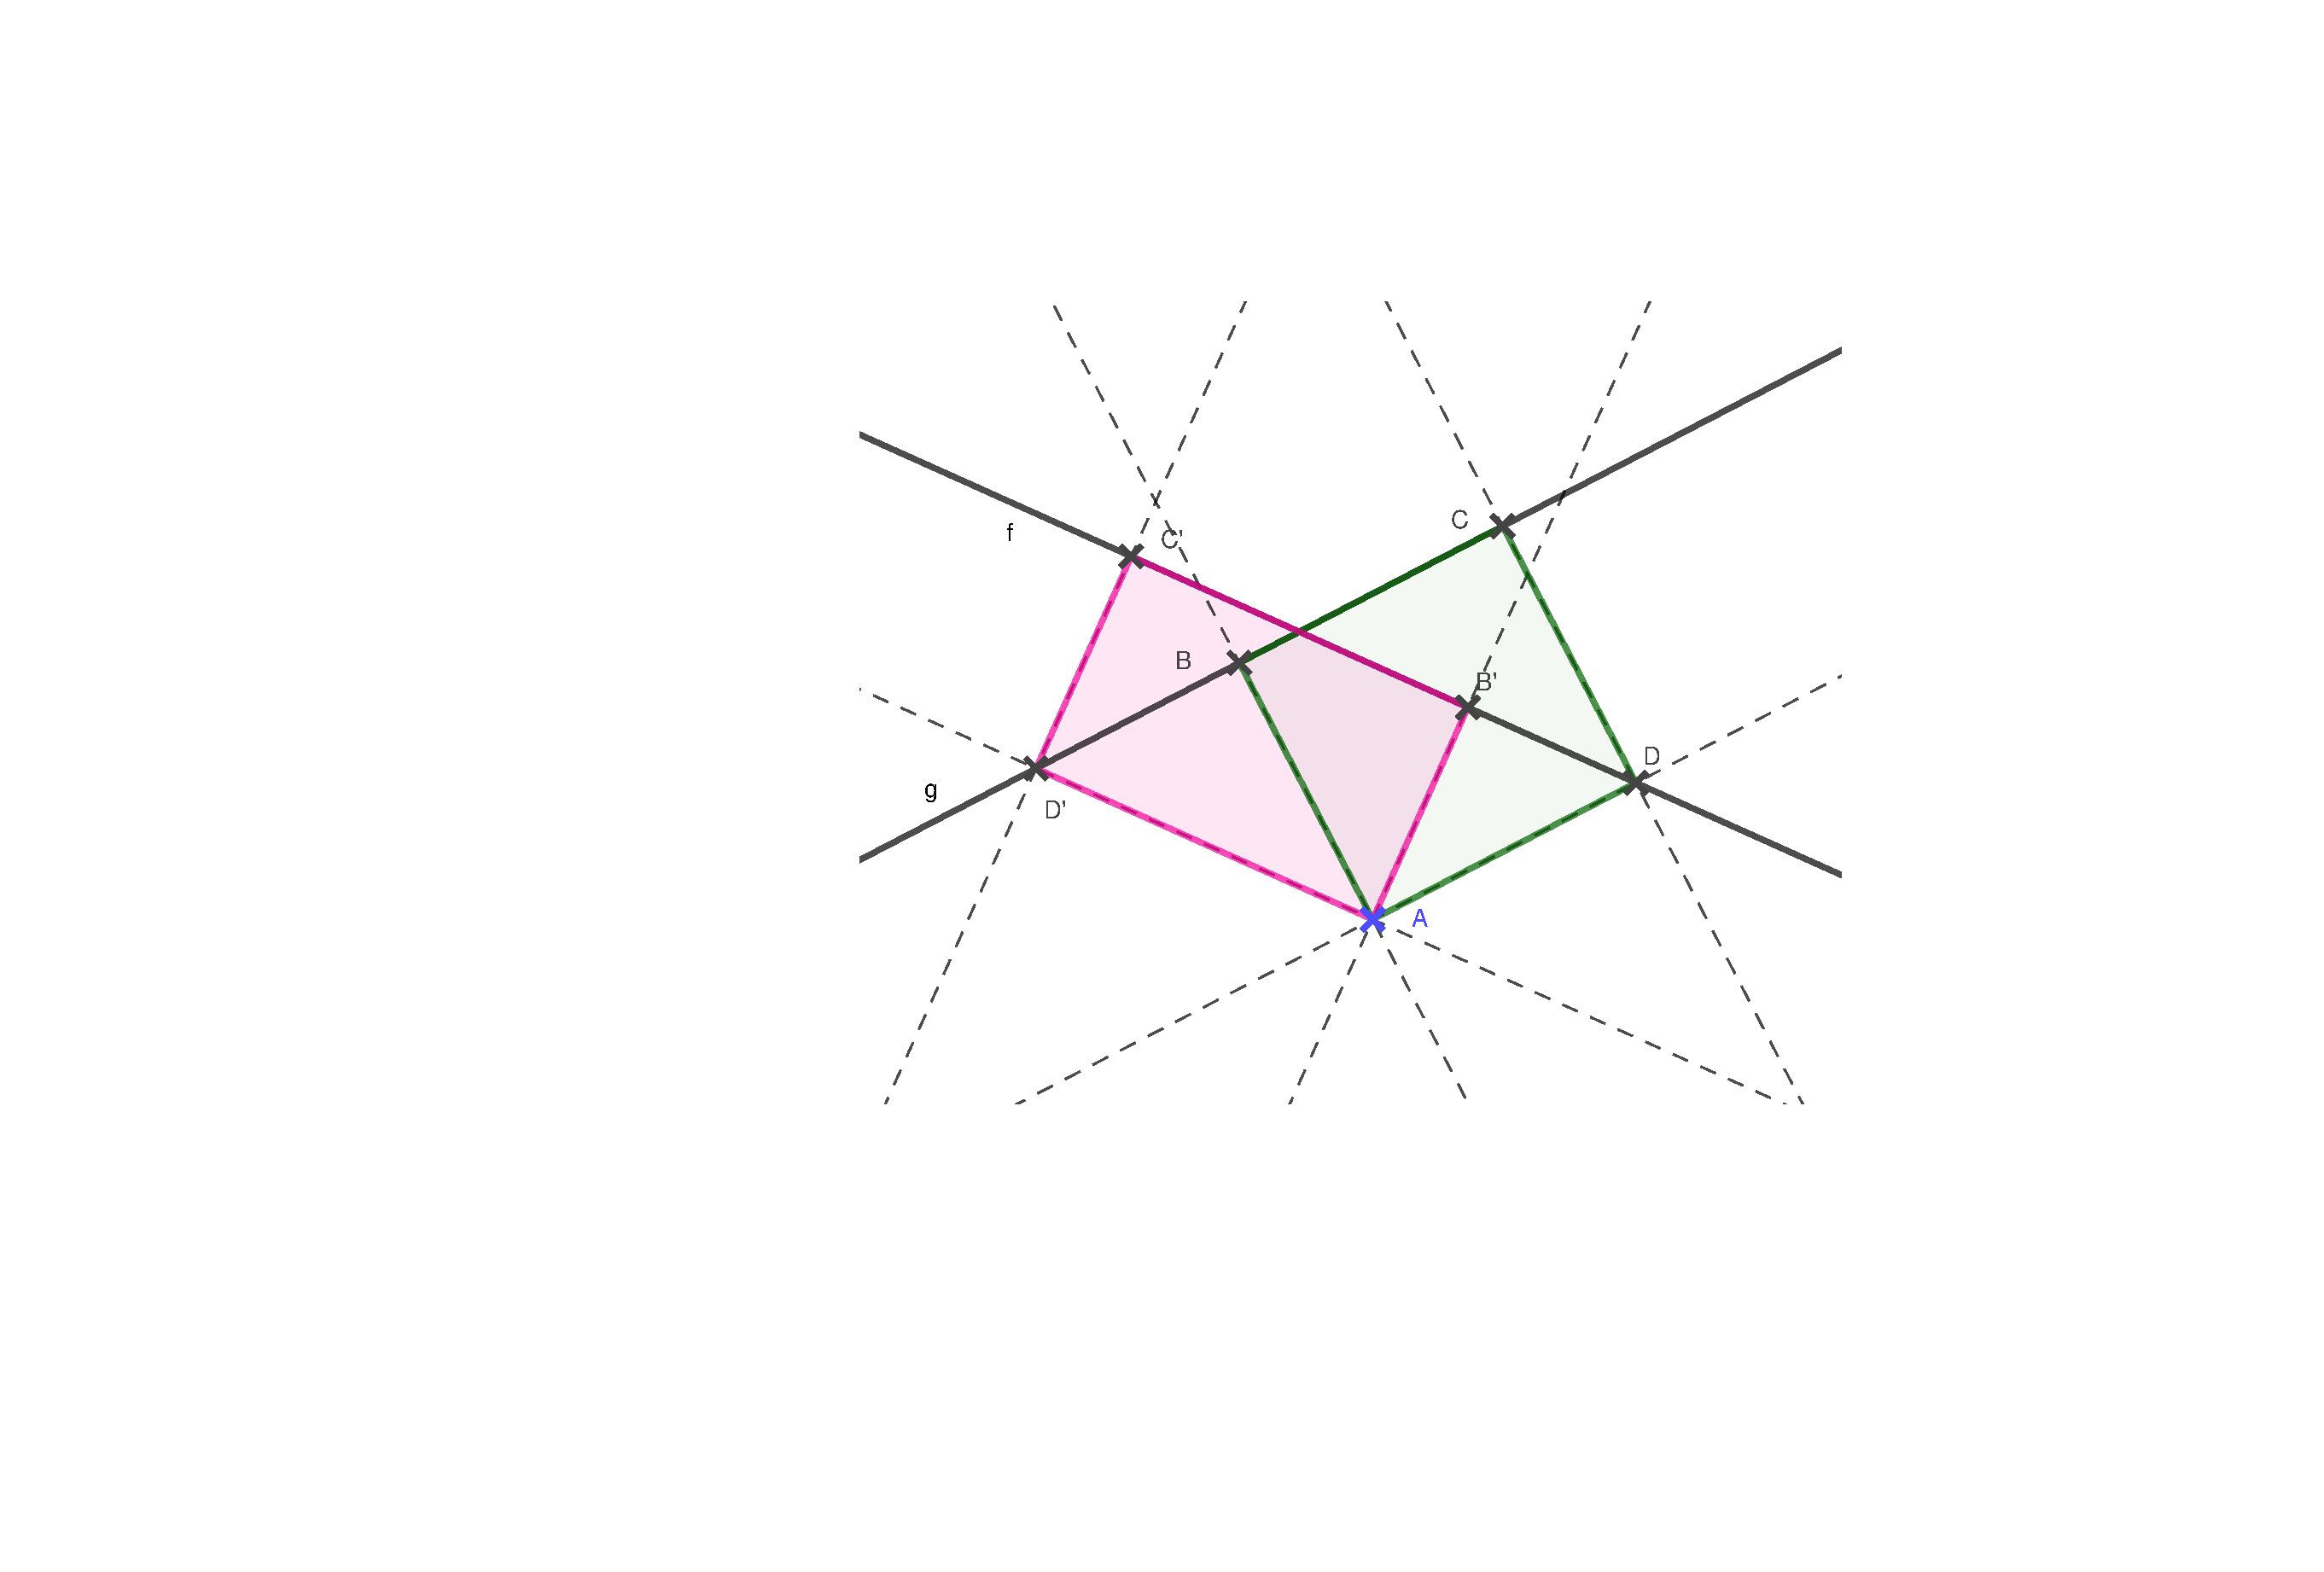
\includegraphics[width=0.6\textwidth]{úlohy/8/rysovani/b/5-v}

    \end{minipage}

    \item
    \begin{minipage}[t]{\linewidth}
        \begin{quote}
            \phantom{text}
        \end{quote}
        \centering
        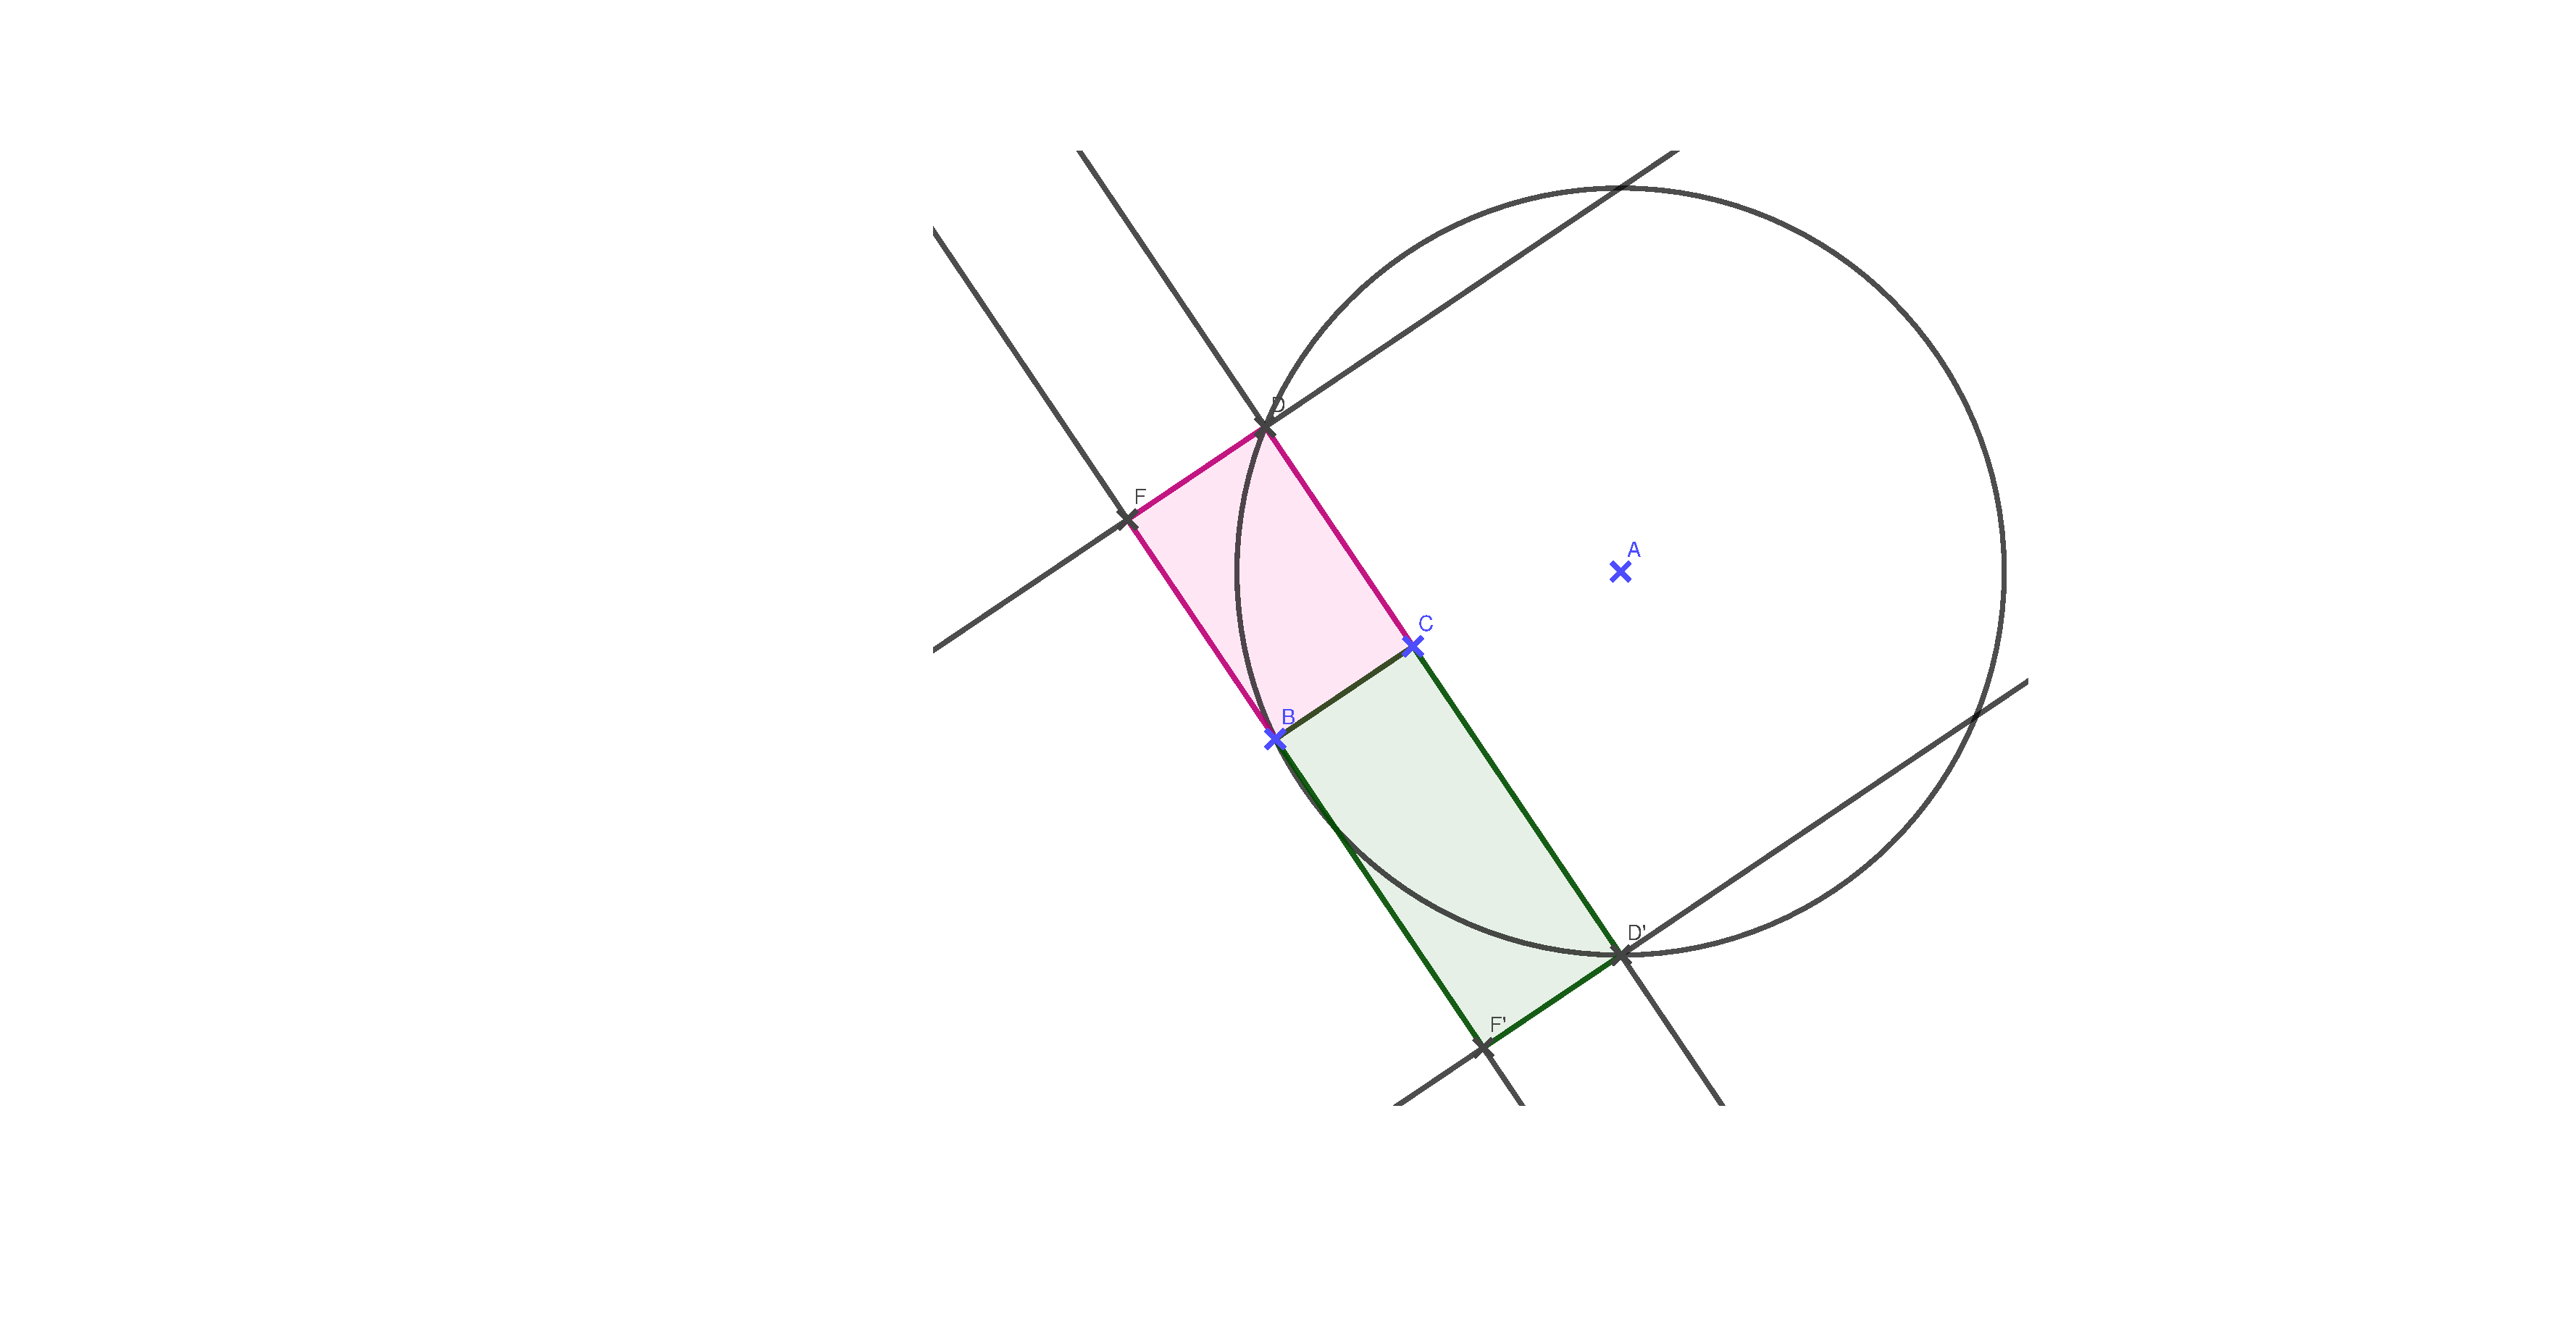
\includegraphics[width=0.6\textwidth]{úlohy/8/rysovani/b/6-v}

    \end{minipage}
\end{enumerate}

\newpage

\subsubsection{Podle bodů a čar}

\paragraph{Úlohy}
\begin{enumerate}
    \item
    \begin{minipage}[t]{\linewidth}
        \begin{quote}
            Narýsujte rovnoramenný $\triangle$ABC, jehož základna leží na $\overleftrightarrow{\text{g}}$.
            Platí, že $\lvert \overleftrightarrow{\text{f}} \text{A} \rvert = \lvert \overleftrightarrow{\text{f}} \text{B} \rvert$.
        \end{quote}
        \centering
        \includegraphics[width=0.8\textwidth]{úlohy/8/rysovani/bp/1}

    \end{minipage}

    \item
    \begin{minipage}[t]{\linewidth}
        \begin{quote}
            Narýsujte $\rectangle$ABCD tak, aby bod C ležel na $\overleftrightarrow{\text{g}}$ a bod D na $\overleftrightarrow{\text{f}}$.
        \end{quote}
        \centering
        \includegraphics[width=0.8\textwidth]{úlohy/8/rysovani/bp/2}

    \end{minipage}

    \item
    \begin{minipage}[t]{\linewidth}
        \begin{quote}
            Narýsujte rovnoramenný $\triangle$ABC, jehož základna leží na $\overleftrightarrow{\text{f}}$.
            Platí $\lvert \overline{\text{XY}} \rvert = \lvert \overline{\text{SB}} \rvert$.
        \end{quote}
        \centering
        \includegraphics[width=0.6\textwidth]{úlohy/8/rysovani/bp/3}

    \end{minipage}

    \item
    \begin{minipage}[t]{\linewidth}
        \begin{quote}
            Narýsujte rovnoramenný $\triangle$ABC, jehož základna leží na $\overleftrightarrow{\text{f}}$.
            Následně vytvořte rovnostranný $\triangle{\text{CDE}}$ tak, aby $\overline{\text{AB}} \perp \overline{\text{CD}}$ a bod E nenáležel $\triangle$ABC\@.
        \end{quote}
        \centering
        \includegraphics[width=0.7\textwidth]{úlohy/8/rysovani/bp/4}

    \end{minipage}

    \item
    \begin{minipage}[t]{\linewidth}
        \begin{quote}
            Sestrojte $\square$ABCD tak, aby bod D ležel na jedné z přímek a aby strana B byla kolmá na druhou.
            Narýsujte všechny možnosti.
        \end{quote}
        \centering
        \includegraphics[width=0.7\textwidth]{úlohy/8/rysovani/bp/5}

    \end{minipage}

    \item
    \begin{minipage}[t]{\linewidth}
        \begin{quote}
            Narýsujte $\rectangle$ABCD tak, aby strana b ležela na $\overrightarrow{\text{XY}}$, ${\lvert \overrightarrow{\text{XY}} \text{A} \rvert = \lvert \text{AZ} \rvert}$ a ${\lvert \text{BC} \rvert = \lvert \text{BZ} \rvert}$.
        \end{quote}
        \centering
        \includegraphics[width=0.8\textwidth]{úlohy/8/rysovani/bp/6}

    \end{minipage}

    \item
    \begin{minipage}[t]{\linewidth}
        \begin{quote}
            Narýsujte $\rectangle$ABCD tak, aby středem $\overline{\text{YZ}}$ byl zároveň středem $\overline{\text{BC}}$.
        \end{quote}
        \centering
        \includegraphics[width=0.8\textwidth]{úlohy/8/rysovani/bp/7}

    \end{minipage}

    \item
    \begin{minipage}[t]{\linewidth}
        \begin{quote}
            Narýsujte rovnoramenný $\triangle$ABC tak, aby bod B ležel na $\overline{\text{ZY}}$, $\lvert \text{SB} \rvert = \lvert \text{SA} \rvert$.
            Základnou je strana BC\@.
        \end{quote}
        \centering
        \includegraphics[width=0.8\textwidth]{úlohy/8/rysovani/bp/8}

    \end{minipage}

    \item
    \begin{minipage}[t]{\linewidth}
        \begin{quote}
            Narýsujte pravoúhlý $\triangle$ABC aby bod B ležel na $\overline{\text{ZY}}$ a strana AC byla jeho nejdelší stranou.

            Dále narýsujte $\triangle$ACD jehož pravý úhel leží u bodu A aby platilo $\lvert \text{AB} \rvert = \lvert \text{AD} \rvert$.

            Jako poslední narýsujte rovnostranný $\triangle$CED tak, aby ${\lvert \text{ED} \rvert > \lvert \text{EA} \rvert}$.
        \end{quote}
        \centering
        \includegraphics[width=0.8\textwidth]{úlohy/8/rysovani/bp/9}

    \end{minipage}

    \item
    \begin{minipage}[t]{\linewidth}
        \begin{quote}
            Narýsujte $\square$ABCD kterým prochází $\overleftrightarrow{\text{f}}$.

            Dále sestrojte $\triangle$EDF tak, aby se bod E nacházel na průsečíku $\overleftrightarrow{\text{f}}$ a $\overleftrightarrow{\text{CD}}$, bod F se nacházel na $\overleftrightarrow{\text{AC}}$ a $\lvert \text{AF} \rvert = \lvert \text{AC} \rvert$.
        \end{quote}
        \centering
        \includegraphics[width=0.8\textwidth]{úlohy/8/rysovani/bp/10}

    \end{minipage}

    \item
    \begin{minipage}[t]{\linewidth}
        \begin{quote}
            Narýsujte $\triangle$ABH aby $\lvert \text{BH} \rvert = \lvert \text{ED} \rvert$, $\lvert \text{AH} \rvert < \lvert \text{EF} \rvert$ a aby se bod H nacházel na lomené čáře CDEFG\@.
        \end{quote}
        \centering
        \includegraphics[width=0.8\textwidth]{úlohy/8/rysovani/bp/11}

    \end{minipage}
\end{enumerate}


\newpage

\paragraph{Řešení}
\begin{enumerate}
    \item
    \begin{minipage}[t]{\linewidth}
        \begin{quote}
            \phantom{text}
        \end{quote}
        \centering
        \includegraphics[width=0.6\textwidth]{úlohy/8/rysovani/bp/1-v}

    \end{minipage}

    \item
    \begin{minipage}[t]{\linewidth}
        \begin{quote}
            \phantom{text}
        \end{quote}
        \centering
        \includegraphics[width=0.6\textwidth]{úlohy/8/rysovani/bp/2-v}

    \end{minipage}

    \item
    \begin{minipage}[t]{\linewidth}
        \begin{quote}
            \phantom{text}
        \end{quote}
        \centering
        \includegraphics[width=0.6\textwidth]{úlohy/8/rysovani/bp/3-v}

    \end{minipage}

    \item
    \begin{minipage}[t]{\linewidth}
        \begin{quote}
            \phantom{text}
        \end{quote}
        \centering
        \includegraphics[width=0.6\textwidth]{úlohy/8/rysovani/bp/4-v}

    \end{minipage}

    \item
    \begin{minipage}[t]{\linewidth}
        \begin{quote}
            \phantom{text}
        \end{quote}
        \centering
        \includegraphics[width=0.6\textwidth]{úlohy/8/rysovani/bp/5-v}

    \end{minipage}

    \item
    \begin{minipage}[t]{\linewidth}
        \begin{quote}
            \phantom{text}
        \end{quote}
        \centering
        \includegraphics[width=0.6\textwidth]{úlohy/8/rysovani/bp/6-v}

    \end{minipage}

    \item
    \begin{minipage}[t]{\linewidth}
        \begin{quote}
            \phantom{text}
        \end{quote}
        \centering
        \includegraphics[width=0.6\textwidth]{úlohy/8/rysovani/bp/7-v}

    \end{minipage}

    \item
    \begin{minipage}[t]{\linewidth}
        \begin{quote}
            \phantom{text}
        \end{quote}
        \centering
        \includegraphics[width=0.6\textwidth]{úlohy/8/rysovani/bp/8-v}

    \end{minipage}

    \item
    \begin{minipage}[t]{\linewidth}
        \begin{quote}
            \phantom{text}
        \end{quote}
        \centering
        \includegraphics[width=0.6\textwidth]{úlohy/8/rysovani/bp/9-v}

    \end{minipage}

    \item
    \begin{minipage}[t]{\linewidth}
        \begin{quote}
            \phantom{text}
        \end{quote}
        \centering
        \includegraphics[width=0.6\textwidth]{úlohy/8/rysovani/bp/10-v}

    \end{minipage}

    \item
    \begin{minipage}[t]{\linewidth}
        \begin{quote}
            \phantom{text}
        \end{quote}
        \centering
        \includegraphics[width=0.6\textwidth]{úlohy/8/rysovani/bp/11-v}

    \end{minipage}
\end{enumerate}


\newpage

\subsection{Stereometrie}
\label{subsec:stereometrie}

\subsubsection{Kostky}

\paragraph{Úlohy}
\begin{enumerate}
    \item
    \begin{minipage}[t]{\linewidth}
        \begin{quote}
            Víte že se kostky dotýkají pouze stěnami. Spočítejte
            \begin{itemize}
                \item počet kostek které jsou vidět,
                \item počet kostek,
                \item počet stěn kostek, které jsou na povrch útvaru,
                \item objem útvaru, pokud je objem jedné kostky 4 cm$^{3}$.
            \end{itemize}
        \end{quote}
        \centering
        \includegraphics[width=0.5\textwidth]{úlohy/8/stereo/1}
    \end{minipage}

    \item
    \begin{minipage}[t]{\linewidth}
        \begin{quote}
            Na obrázku vidíte stavbu složenou z krychlí. Jak může vypadat z druhé strany? Vyberte všechny možnosti.
        \end{quote}
        \centering
        \includegraphics[width=0.6\textwidth]{úlohy/8/stereo/2}
    \end{minipage}

    \item
    \begin{minipage}[t]{\linewidth}
        \begin{quote}
			Pojmenujte tělesa zleva doprava.
        \end{quote}
        \centering
        \includegraphics[width=0.6\textwidth]{úlohy/8/stereo/3}
    \end{minipage}

    \item
    \begin{minipage}[t]{\linewidth}
        \begin{quote}
			Kolik je na obrázku nejmenší možný počet kostek, pokud víme, že kostka musí stát buď na podložce nebo na jiné kostce?
        \end{quote}
        \centering
        \includegraphics[width=0.6\textwidth]{úlohy/8/stereo/4}
    \end{minipage}

    \item
    \begin{minipage}[t]{\linewidth}
        \begin{quote}
			Vlevo je těleso složené z kostek. Jak by mohlo vypadat, pokud by jsme se na něj podívali z určité strany? Vyberte možné pohledy zprava. (Vyber A, B, C nebo D.)
        \end{quote}
        \centering
        
        \includegraphics[width=0.45\textwidth]{úlohy/8/stereo/5}
        \includegraphics[width=0.5\textwidth]{úlohy/8/stereo/5-1}
    \end{minipage}

    \item
    \begin{minipage}[t]{\linewidth}
        \begin{quote}
			Srovnejte tělesa složená z kostek podle obsahu. Určete, o kolik cm$^{3}$ je největší těleso větší než nejmenší těleso, pokud je obsah jedné kostky 3 cm$^{3}$.
        \end{quote}
        \centering
        \includegraphics[width=0.9\textwidth]{úlohy/8/stereo/6}
    \end{minipage}

    \item
    \begin{minipage}[t]{\linewidth}
        \begin{quote}
			Na obrázku je písmeno H slepené z bílých kostek. Po slepení bylo namalováno na žluto.
			
			Kolik stěn na sobě má lepidlo? kolik stěn má na sobě žlutou barvu.
        \end{quote}
        \centering
        \includegraphics[width=0.4\textwidth]{úlohy/8/stereo/7}
    \end{minipage}

    \item
    \begin{minipage}[t]{\linewidth}
        \begin{quote}
			Na obrázku jsou poskládány hrací kostky do útvaru. Víme, že 
			\begin{itemize}
				\item součet hodnot dvou protějších stran hrací kostky je 7.
				\item Všechny kostky se dotýkají stěnami,
				\item kostka která není vidět byla posunuta doleva.
				\item Tři tečky se šipkou ukazují jaká hodnota je na spodní stěně pravé dolní kostky.
				\item Některé hodnoty jsou neznámé, ty jsou označené otazníkem.
			\end{itemize}
			
			Jaký je součet všech hodnot, které jsou na útvaru zvenku?
        \end{quote}
        \centering
        \includegraphics[width=0.55\textwidth]{úlohy/8/stereo/8}
    \end{minipage}

    \item
    \begin{minipage}[t]{\linewidth}
        \begin{quote}
			Na horní obrázku jsou kostky. Dotýkají se buď stěnami nebo hranami.
			
			Do čtvercových sítí vkresli co bychom viděli pokud bychom se dívali na kostky z 2 úhlů podhledu. Do pravé to co bychom viděli shora, a do levé to co bychom viděli zleva.
        \end{quote}
        \centering
        \includegraphics[width=0.6\textwidth]{úlohy/8/stereo/9-1}
        \includegraphics[width=0.6\textwidth]{úlohy/8/stereo/9-2}
    \end{minipage}

    \item
    \begin{minipage}[t]{\linewidth}
        \begin{quote}
			Zelené kostky byly slepené lepidlem do tělesa nahoře. Kvůli horku se těleso roztálo, a všechny kostky spadly.
			
			Jak kostky po spadnutí vypadají? (Vyber A, B, nebo C.)
        \end{quote}
        \centering
        \includegraphics[width=0.7\textwidth]{úlohy/8/stereo/10}
    \end{minipage}

    \item
    \begin{minipage}[t]{\linewidth}
        \begin{quote}
			Na obrázku je narozeninový dort focený shora. Má 3 patra, nejnižší je modré, prostřední je zelené a nejvyšší je hnědé. Do čtvercových sítí dokresli, jak dort vypadá ze stran určených šipkami.
        \end{quote}
        \centering
        \includegraphics[width=0.6\textwidth]{úlohy/8/stereo/11}
    \end{minipage}

    \item
    \begin{minipage}[t]{\linewidth}
        \begin{quote}
			Na obrázku jsou 2 fotky skleněného objektu. Jenda je focená shora, druhá zepředu.
			
			Popište tento objekt. (Možný popis: Objekt je na povrchu modrý a má tvar koule, uvnitř této koule je zelený čtverec.)
        \end{quote}
        \centering
        \includegraphics[width=0.6\textwidth]{úlohy/8/stereo/12}
    \end{minipage}

\end{enumerate}

\newpage

\paragraph{Řešení}
\begin{enumerate}
    \item
    \begin{quote}
        Kostek je vidět 6. Pokud víme že se kostky dotýkají, je jich 7. Na povrchu útvaru je 30 stěn. Objem je 28 cm$^{3}$.
    \end{quote}

    \item
    \begin{quote}
        Může vypadat jako A nebo B.
    \end{quote}

    \item
    \begin{quote}
		Tělesa se jmenují kostka, válec a jehlan.
    \end{quote}

    \item
    \begin{quote}
		Je na něm minimálně 14 kostek.
    \end{quote}

    \item
    \begin{quote}
		Může vypadat jako možnost A, B a D.
    \end{quote}

    \item
    \begin{quote}
		Největší je prostřední těleso, druhé největší je těleso vlevo a nejmenší je těleso vpravo. Největší těleso je větší než nejmenší těleso o 171 cm$^{3}$.
    \end{quote}

    \item
    \begin{quote}
		22 stěn na sobě má lepidlo, 50 stěn na sobě má žlutou barvu.
    \end{quote}

    \item
    \begin{quote}
		Součet je 115.
    \end{quote}

    \item
    \begin{minipage}[t]{\linewidth}
    	\begin{quote}
    		\phantom{text}
    	\end{quote}
    	\centering
    	\includegraphics[width=0.6\textwidth]{úlohy/8/stereo/9-v}
    \end{minipage}

    \item
    \begin{quote}
		Správná možnost je C.
    \end{quote}

    \item
    \begin{minipage}[t]{\linewidth}
    	\begin{quote}
    		\phantom{text}
    	\end{quote}
    	\centering
    	\includegraphics[width=0.6\textwidth]{úlohy/8/stereo/11-v}
    	\begin{quote}
    		3d vizualizace:
    	\end{quote}
    	\centering
    	\includegraphics[width=0.6\textwidth]{úlohy/8/stereo/11-v-3d}
    \end{minipage}

    \item
    \begin{quote}
		Objekt je na povrchu oranžový a má tvar válce, uvnitř tohoto válce je modrý jehlan.
    \end{quote}
\end{enumerate}